%==============================================================================
% AI6127 Deep Neural Networks for NLP -- Group Assignment Report, Group 13
% Experimental-report (paper) layout: two columns, Times.
%
% Build:  latexmk -xelatex main.tex   then copy main.pdf to 13.pdf
%         (XeLaTeX is needed only for the Chinese queries in Appendix C.)
%
% The brief (docs/Assignment.pdf) asks for:
%   - names AND matriculation numbers of all members on the first page
%   - answers to Questions 1-5     (mapping: Table 1 in the Introduction)
%   - a Drive/OneDrive link to the data zip and one to the code zip
%   - a single PDF named "13.pdf" (Word or zip = demerit points)
% Placeholders still to fill are marked with \tbd{...} (orange boxes).
%==============================================================================
\documentclass[10pt,twocolumn,a4paper]{article}

\usepackage[a4paper,margin=0.75in,columnsep=0.25in]{geometry}
\usepackage{newtxmath}
\usepackage{fontspec}
\setmainfont{texgyretermes}[Extension=.otf, UprightFont=*-regular, BoldFont=*-bold,
  ItalicFont=*-italic, BoldItalicFont=*-bolditalic]
\setsansfont{texgyreheros}[Extension=.otf, UprightFont=*-regular, BoldFont=*-bold,
  ItalicFont=*-italic, BoldItalicFont=*-bolditalic, Scale=MatchLowercase]
\setmonofont{texgyrecursor}[Extension=.otf, UprightFont=*-regular, BoldFont=*-bold,
  ItalicFont=*-italic, BoldItalicFont=*-bolditalic]
\usepackage{xeCJK}
\setCJKmainfont{Songti SC}[AutoFakeSlant=0.18]

\usepackage[table]{xcolor}
\usepackage{graphicx}
\usepackage{booktabs,tabularx,array,multirow}
\usepackage[group-separator={,},group-minimum-digits=4]{siunitx}
\usepackage{amsmath}
\usepackage{enumitem}
\setlist{itemsep=1pt,topsep=3pt,parsep=0pt,leftmargin=1.2em}
\usepackage{caption}
\captionsetup{font=small}
\usepackage{subcaption}
\usepackage{pgfplots}
\pgfplotsset{compat=1.18}
\usetikzlibrary{positioning,arrows.meta,calc}
\usepackage{fancyvrb}
\usepackage[style=numeric-comp,sorting=none,maxbibnames=3,backend=biber,urldate=iso,seconds=true]{biblatex}
\addbibresource{refs.bib}
\renewcommand*{\bibfont}{\small}
\usepackage{xurl}
\usepackage[hidelinks]{hyperref}
\usepackage[capitalise,nameinlink]{cleveref}
\crefname{section}{Section}{Sections}
\Crefname{section}{Section}{Sections}

% placeholders to be filled before submission
\definecolor{tbdbg}{HTML}{FBE3CF}
\definecolor{tbdfg}{HTML}{A0410D}
\newcommand{\tbd}[1]{\colorbox{tbdbg}{\footnotesize\color{tbdfg}#1}}
\newcommand{\best}[1]{\textbf{#1}}
\newcolumntype{P}[1]{>{\raggedright\arraybackslash}p{#1}}
\newcolumntype{Y}{>{\raggedright\arraybackslash}X}
\definecolor{shade}{HTML}{EEEEEE}

% chart style: sans ticks, recessive grid, validated series colours
\definecolor{s1}{HTML}{2A78D6}
\definecolor{s2}{HTML}{EB6834}
\definecolor{s3}{HTML}{1BAF7A}
\definecolor{s4}{HTML}{EDA100}
\definecolor{gridc}{HTML}{E3E3E3}
\definecolor{axisc}{HTML}{777777}
\pgfplotsset{
  barlegend/.style={legend image code/.code={\fill[##1] (0pt,-2.5pt) rectangle (6pt,3.5pt);}},
  paper/.style={
    font=\sffamily\scriptsize, axis line style={draw=axisc}, tick style={draw=axisc},
    major grid style={draw=gridc}, ymajorgrids, tick label style={color=black!75},
    legend style={draw=none, fill=none, font=\sffamily\scriptsize, legend columns=-1,
      /tikz/every even column/.append style={column sep=6pt}},
    legend cell align=left, title style={font=\sffamily\scriptsize\bfseries},
    xticklabel={\pgfmathprintnumber[assume math mode=true]{\tick}},
    yticklabel={\pgfmathprintnumber[assume math mode=true]{\tick}}},
}

\title{\bfseries Ask the Reviews: Grounded, Constraint-Aware\\
       Question Answering over 61{,}167 Airline Passenger Reviews}

\author{%
\begin{tabular}{@{}c@{\hspace{2.2em}}c@{\hspace{2.2em}}c@{}}
Ren Xinghan & Sun Sijie & Zhang Yuxuan \\
\small Matric.\ No.\ \tbd{to fill} & \small Matric.\ No.\ G2600457L & \small Matric.\ No.\ G2606145J \\[6pt]
Zhu Jindou & Guo Tailai & Sun Yuxin \\
\small Matric.\ No.\ G2609499B & \small Matric.\ No.\ G2602966F & \small Matric.\ No.\ \tbd{to fill} \\
\end{tabular}\\[10pt]
AI6127 Deep Neural Networks for NLP\,---\,Group 13\\
Nanyang Technological University}
\date{7 November 2026}

\begin{document}
\maketitle

%------------------------------------------------------------------ Abstract
\begin{abstract}
We address question answering over passenger reviews for travellers choosing an airline. Real questions are
constrained (a route, a cabin, a traveller type), they ask about fine-grained attributes such as legroom or seat
cleanliness that structured ratings do not cover, and they need a verdict the user can check. We build a
retrieval-augmented system over \num{61167} Skytrax reviews split into \num{546139} sentence passages. The query is
parsed into hard metadata filters and one of 46 sub-attributes; evidence is retrieved with BM25 and MiniLM dense search
fused by reciprocal rank fusion; an offline sentence classifier labels subjectivity, polarity and aspect so that the
verdict is a count over \emph{every} matching review; and a local Qwen3-4B model writes a cited answer that program
guards accept only if its citations, numbers and direction agree with the evidence. On 30 airline $\times$
sub-attribute queries the hybrid retriever reaches NDCG@10 0.810 and MRR 0.961, while a general-purpose cross-encoder
\emph{lowers} NDCG@10 by 0.066 (95\% CI $[-0.114,-0.019]$). Replacing the rule-based classifier with a linear student trained on weak labels plus
labels distilled from an LLM raises three-class macro-F1 on our \num{1000}-sentence human-labelled set from 57.2 to 78.5 and joint aspect--polarity accuracy
by 7.4 points (CI $[+4.5,+10.4]$), while relabelling the whole corpus in 18\,s. On 20 end-to-end questions the guarded
system scores 0.84 faithfulness and 0.99 answer relevance, with 16 of the 20 final answers written by the program
fallback. A full factorial ablation of the three answer-side
components (160 answers) finds balanced evidence plus validation the most faithful configuration ($+0.053$, CI
$[+0.004,+0.106]$) and shows that their gains are not additive. Text-derived airline rankings agree with
held-out passenger ratings (Spearman $\rho=0.81$ over 58 airlines). Everything runs locally at zero API cost.
\end{abstract}

%-------------------------------------------------------------- Introduction
\section{Introduction}
\label{sec:intro}

A traveller deciding between airlines does not ask ``what do reviews say about seats?''. They ask ``flying Singapore
to London in economy, which airline has the best legroom?'', or ``how clean are Singapore Airlines seats?''. Such
questions combine hard constraints with an attribute that is usually mentioned only in free text, and the answer is
only useful if the user can see how much evidence lies behind it and check it. Review sites hold this evidence, but in
tens of thousands of long reviews that no one can read before booking.

We frame the task as retrieval-augmented opinion question answering, and derive three requirements that shape the
whole design:
\begin{enumerate}[label=\textbf{R\arabic*}]
  \item \textbf{Constraints must hold.} Route, cabin, traveller type and date are filters on the evidence, not hints to a ranker.
  \item \textbf{Fine-grained attributes need text.} The data rates only six coarse aspects; legroom, recline or meal portion size appear only in the review text.
  \item \textbf{The verdict must be traceable.} The overall direction is computed over all matching reviews, and every claim in an answer cites a review sentence.
\end{enumerate}

\noindent The contributions of this report are:
\begin{itemize}
  \item A cleaned, sentence-level knowledge base with structured metadata, and an audit of the data problems that would otherwise damage retrieval (\cref{sec:kb}).
  \item A retrieval pipeline that turns constraints into filters and routes 46 sub-attributes with query expansion, evaluated with rank-aware metrics and bootstrap intervals, including a negative result for cross-encoder reranking (\cref{sec:method,sec:exp-ret}).
  \item A distillation protocol that moves an LLM labeller into a fast classifier with pre-registered selection that never reads the gold set (\cref{sec:exp-distill}).
  \item Three answer-side components (full-pool statistics, balanced and label-consistent evidence, validation with repair and fallback) evaluated in a full $2^3$ factorial ablation, and an airline-ranking validation against held-out passenger ratings (\cref{sec:exp-abl,sec:exp-rank}).
\end{itemize}

\noindent The brief poses five questions; \cref{tab:map} shows where each is answered.

\begin{table}[t]
\centering\small
\caption{Where each question of the assignment brief is answered.}
\label{tab:map}
\begin{tabularx}{\columnwidth}{@{}lYl@{}}
\toprule
\textbf{Q} & \textbf{Topic} & \textbf{Sections} \\
\midrule
Q1 & Corpus gathering, cleaning, chunking, storage, application, statistics & \S\ref{sec:kb} \\
Q2 & User interface; five queries and their speed & \S\ref{sec:ui}, \S\ref{sec:exp-speed} \\
Q3 & Retrieval innovations; rank-aware evaluation & \S\ref{sec:ret}, \S\ref{sec:exp-ret} \\
Q4 & Approach, evaluation dataset, classification and RAG metrics, performance & \S\ref{sec:cls}, \S\ref{sec:data}, \S\ref{sec:exp-cls}, \S\ref{sec:exp-rag}, \S\ref{sec:exp-perf} \\
Q5 & Downstream innovations; ablation studies & \S\ref{sec:gen}, \S\ref{sec:exp-distill}, \S\ref{sec:exp-abl}, \S\ref{sec:exp-rank} \\
\bottomrule
\end{tabularx}
\end{table}

%------------------------------------------------------------- Related work
\section{Related Work}
\label{sec:related}

\paragraph{Retrieval.} Sparse retrieval with BM25~\cite{bm25} remains a strong baseline; dense bi-encoders such as
Sentence-BERT~\cite{sbert} with MiniLM~\cite{minilm} capture paraphrases and are searched efficiently with
FAISS~\cite{faiss}. Reciprocal rank fusion~\cite{rrf} combines rankings without calibrating scores, and cross-encoders
trained on MS MARCO~\cite{msmarco,nogueira2019} are the usual second-stage rerankers. We evaluate with
NDCG~\cite{ndcg} and related rank-aware metrics.

\paragraph{Aspect-based sentiment.} Aspect-based sentiment analysis~\cite{pontiki2014} has moved from lexicon and rule
systems such as SenticNet~\cite{senticnet} to fine-tuned transformers~\cite{xu2019bert} and to zero-shot prompting of
large language models. LLM labels can replace part of the human annotation effort~\cite{gilardi2023}, and knowledge
distillation~\cite{hinton2015} transfers an expensive model's behaviour into a cheaper one.

\paragraph{Grounded generation.} Retrieval-augmented generation~\cite{rag} conditions a generator on retrieved
passages; RAGAS~\cite{ragas} defines reference-free answer metrics (faithfulness, answer relevance, context
precision) that we adopt.

%------------------------------------------------------- Knowledge base (Q1)
\section{Knowledge Base Construction}
\label{sec:kb}

\paragraph{Source.} The corpus is the public Skytrax review collection released on Kaggle
(\nolinkurl{efehandanisman/skytrax-airline-reviews})~\cite{skytraxkaggle}. Each record holds the review text with
airline, cabin, traveller type, route, date flown, aircraft, six 1--5 aspect ratings (seat comfort, cabin service, food
and beverages, entertainment, ground service, value for money), a 1--10 overall score and a recommend flag. We download
it with \texttt{kagglehub}; no scraping is involved.

\paragraph{Why this domain.} The brief asks for enough data and a balanced task. Opinions are mixed within and across
airlines (40\% of opinionated gold sentences are positive, 60\% negative), and the ratings give free weak supervision.
We rejected paper peer reviews (too hedged for 80\% inter-annotator agreement), MOOC reviews (overwhelmingly five-star),
cryptocurrency (the brief's own example, swinging with the market) and Steam reviews (the most likely to overlap with
other groups).

\paragraph{Cleaning.} We audited all \num{65947} non-empty reviews before writing cleaning code; \cref{tab:cleaning}
lists what we found. Two problems affected over 40\% of reviews. We deliberately did \emph{not} lower-case, strip
punctuation or correct spelling: the text is shown to users as evidence, and exclamation marks and intensifiers are
sentiment signals. Lower-casing happens only inside the BM25 index.

\begin{table*}[t]
\centering\small
\caption{Data problems found in the raw corpus and how they were fixed (\nolinkurl{src/clean_text.py}).}
\label{tab:cleaning}
\begin{tabularx}{\textwidth}{@{}P{42mm}rY@{}}
\toprule
\textbf{Problem} & \textbf{Share} & \textbf{Example and fix} \\
\midrule
Blank spreadsheet rows & 50.0\% of rows & \num{131895} rows, of which \num{65947} carry a review; the rest are dropped. \\
Mojibake (UTF-8 read as cp1252) & 42.4\% & \texttt{wasn’t}\,$\to$\,\texttt{wasn't}; \texttt{Düsseldorf}\,$\to$\,\texttt{Düsseldorf}. Re-encoding whole reviews left 2.14\% broken, repairing suspicious spans 0.37\%; \texttt{ftfy}~\cite{ftfy} plus a span-level second pass leaves 6 flagged sentences (0.001\%), all genuine Spanish, French or Portuguese. \\
Site boilerplate & 43.5\% & Prefixes \texttt{Trip Verified |} (\num{13670}), \texttt{Verified Review |} (\num{12126}), \texttt{Not Verified |} (\num{1714}) and a trailing \texttt{… Ranking}, removed with anchored patterns; otherwise every query on ``verified'' would match them. \\
Duplicate reviews & 7.2\% & Exact de-duplication: \num{65947}\,$\to$\,\num{61172} unique texts. \\
Too-short reviews & $<$0.01\% & Under 20 characters after cleaning: \num{61172}\,$\to$\,\num{61167}. \\
\bottomrule
\end{tabularx}
\end{table*}

\paragraph{Chunking.} We split every review into sentences with spaCy~\cite{spacy}. A sentence usually carries one
opinion about one aspect, so a retrieval hit, a classifier label and a citation all refer to the same span; longer
windows mix aspects, because a typical review moves from check-in to seat to food (\cref{fig:corpus}, bottom). Each
sentence keeps its \nolinkurl{review_id} and the full review, so the interface can expand a hit to its parent
(parent-document retrieval). Sentences of fewer than three words or five letters are dropped at split time;
\num{16772} route-only lines and 336 non-English sentences are excluded from retrieval (19 sentence fragments are
flagged but kept), leaving a pool of \num{529031} of the \num{546139} sentences.

\paragraph{Storage.} The result is one table, \nolinkurl{data/processed/chunks.parquet} (31 columns: sentence, parent
review, metadata, ratings, route parsed into origin, destination and stop-over, quality flags), which is the single
data contract of all three subgroups. zstd compression reduces it from 96\,MB to 31\,MB. On it we build a BM25 index
(6\,s), a FAISS \texttt{IndexFlatIP} over L2-normalised 384-d \texttt{all-MiniLM-L6-v2} embeddings (4.6\,min, mostly encoding) and the
label index of \cref{sec:cls}. A full rebuild takes about 14 minutes.

\begin{table}[t]
\centering\small
\caption{Corpus statistics after cleaning and chunking. Words are whitespace tokens; types are distinct lower-cased tokens.}
\label{tab:corpus}
\begin{tabular}{@{}lr@{}}
\toprule
Documents (reviews) & \num{61167} \\
Chunks (sentences) & \num{546139} \\
\quad of which retrievable & \num{529031} \\
Words (tokens) & \num{8276082} \\
Types (unique words) & \num{130385} \\
Airlines & 81 \\
Review dates & Aug 2002 -- Jun 2019 \\
Reviews by cabin: Economy & \num{45163} \\
\quad Business / Premium / First & \num{9589} / \num{2411} / \num{1532} \\
\quad Cabin not given & \num{2472} \\
\bottomrule
\end{tabular}
\end{table}

\begin{figure}[t]
\centering
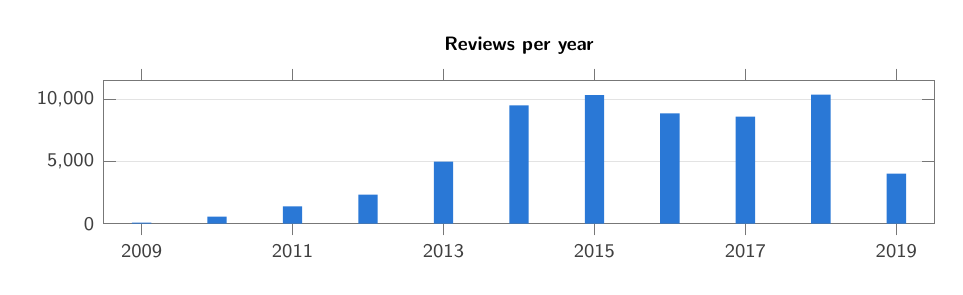
\begin{tikzpicture}
\begin{axis}[paper, width=\columnwidth, height=34mm, ybar, bar width=7pt,
  title={Reviews per year}, xmin=2008.5, xmax=2019.5, ymin=0, ymax=11500,
  xtick={2009,2011,2013,2015,2017,2019}, xticklabel={\pgfmathprintnumber[assume math mode=true,1000 sep=]{\tick}},
  ytick={0,5000,10000}, scaled y ticks=false, yticklabel style={/pgf/number format/1000 sep={,}}, enlargelimits=false]
\addplot[fill=s1, draw=none] coordinates {(2009,94) (2010,569) (2011,1381) (2012,2332) (2013,4987) (2014,9501) (2015,10323) (2016,8864) (2017,8607) (2018,10368) (2019,4026)};
\end{axis}
\end{tikzpicture}\\[2pt]
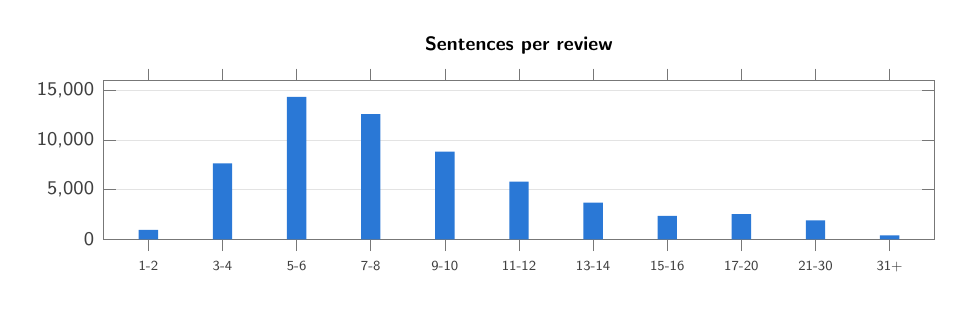
\begin{tikzpicture}
\begin{axis}[paper, width=\columnwidth, height=36mm, ybar, bar width=7pt,
  title={Sentences per review}, symbolic x coords={1-2,3-4,5-6,7-8,9-10,11-12,13-14,15-16,17-20,21-30,31+},
  xtick=data, xticklabel style={font=\sffamily\tiny}, ymin=0, ymax=16000,
  ytick={0,5000,10000,15000}, scaled y ticks=false, yticklabel style={/pgf/number format/1000 sep={,}}, enlarge x limits=0.06]
\addplot[fill=s1, draw=none] coordinates {(1-2,968) (3-4,7650) (5-6,14363) (7-8,12608) (9-10,8840) (11-12,5817) (13-14,3694) (15-16,2366) (17-20,2541) (21-30,1919) (31+,401)};
\end{axis}
\end{tikzpicture}
\caption{Top: review volume grows from 2013 (115 reviews before 2009 omitted); 2019 is partial. Bottom: most reviews
have 5--10 sentences and therefore mix several aspects, which motivates sentence-level passages.}
\label{fig:corpus}
\end{figure}

\paragraph{Statistics.} \Cref{tab:corpus} gives the size of the corpus, well above the required \num{10000} documents
and \num{100000} words. Its main bias is towards economy class (74\% of reviews) and towards large airlines (Spirit,
American, United and British Airways have about \num{2800} reviews each); answers therefore state the number of
matching reviews so users can judge how thin the evidence is.

\paragraph{Application and sample queries.} Users are travellers choosing an airline and analysts comparing service
quality. They ask in English or Chinese, or set filters directly, and receive a cited verdict, a positive/negative tally
over all matching reviews, the rating summary and the evidence. Typical queries: \emph{How is the legroom in Singapore
Airlines economy?} (one sub-attribute); \emph{Flying Singapore to London in economy, which airline has the best
legroom?} (route constraint, open comparison); \emph{Compare Qatar Airways and British Airways business class seat
recline} (two airlines); \emph{Singapore Airlines economy: food, value for money and ground service?} (several
aspects); and the Chinese \emph{阿联酋航空经济舱的退款和改签处理怎么样？} (Emirates refunds and rebooking).

%--------------------------------------------------------------- Method
\section{Proposed System}
\label{sec:method}

\Cref{fig:arch} shows the pipeline. Indexes and labels are built offline; per query, filters are applied before
retrieval, and the generator's draft is accepted only if program checks pass. The system runs on an Apple M1 Pro
laptop with 16\,GB of memory; no hosted RAG service or paid API is used.

\begin{figure*}[t]
\centering
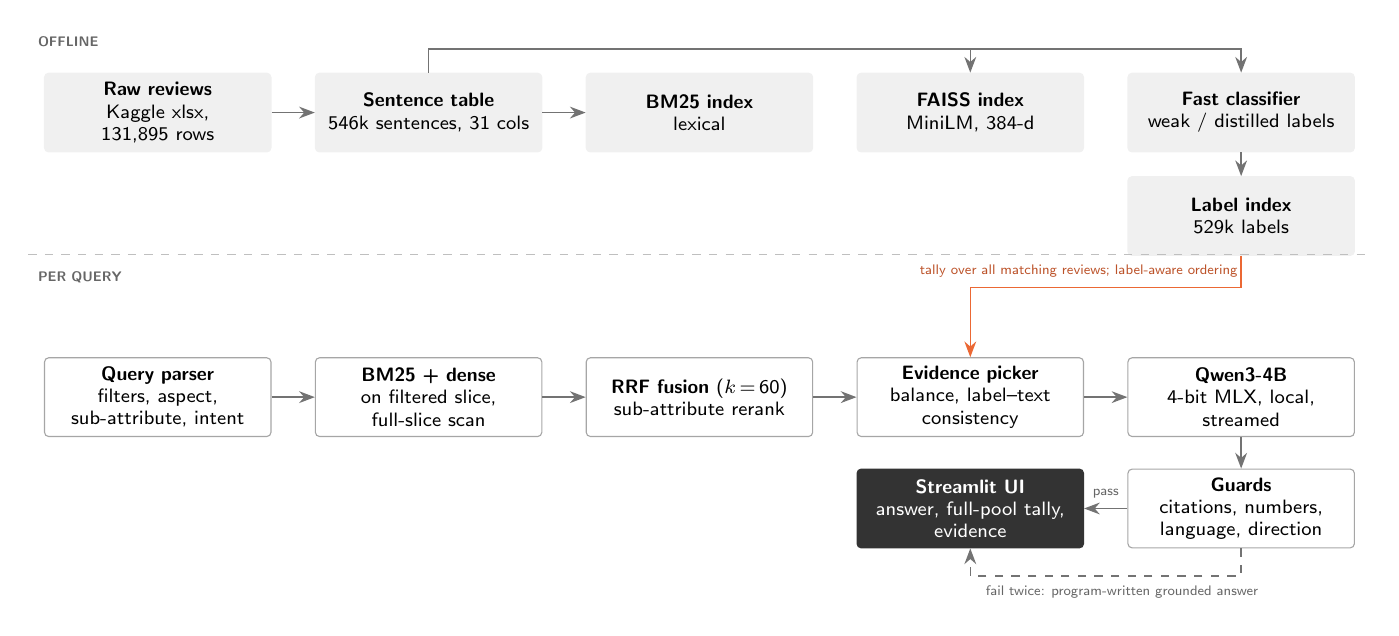
\begin{tikzpicture}[
  font=\sffamily\scriptsize, node distance=4mm and 5.5mm,
  box/.style={draw=black!35, fill=white, rounded corners=1.5pt, align=center, minimum height=10mm, text width=27mm, inner sep=2.5pt},
  off/.style={box, fill=black!6, draw=black!6},
  hot/.style={box, fill=black!80, draw=black!80, text=white},
  arr/.style={-{Stealth[length=2mm]}, draw=black!55, line width=0.55pt},
  lab/.style={font=\sffamily\tiny\bfseries, text=black!60, anchor=west}]
  \node[off] (raw) {\textbf{Raw reviews}\\ Kaggle xlsx, 131,895 rows};
  \node[off, right=of raw] (chunks) {\textbf{Sentence table}\\ 546k sentences, 31 cols};
  \node[off, right=of chunks] (bm25) {\textbf{BM25 index}\\ lexical};
  \node[off, right=of bm25] (faiss) {\textbf{FAISS index}\\ MiniLM, 384-d};
  \node[off, right=of faiss] (cls) {\textbf{Fast classifier}\\ weak / distilled labels};
  \node[off, below=3mm of cls] (labels) {\textbf{Label index}\\ 529k labels};
  \draw[arr] (raw) -- (chunks);
  \draw[arr] (chunks) -- (bm25);
  \draw[arr] (chunks.north) -- ++(0,3mm) -| (faiss.north);
  \draw[arr] (chunks.north) -- ++(0,3mm) -| (cls.north);
  \draw[arr] (cls) -- (labels);
  \draw[dashed, draw=black!25] ($(raw.west)+(-2mm,-18mm)$) -- ($(cls.east)+(2mm,-18mm)$);
  \node[lab] at ($(raw.west)+(-2mm,9mm)$) {OFFLINE};
  \node[lab] at ($(raw.west)+(-2mm,-21mm)$) {PER QUERY};
  \node[box, below=26mm of raw] (q) {\textbf{Query parser}\\ filters, aspect,\\ sub-attribute, intent};
  \node[box, right=of q] (ret) {\textbf{BM25 + dense}\\ on filtered slice,\\ full-slice scan};
  \node[box, right=of ret] (rrf) {\textbf{RRF fusion} ($k$\,=\,60)\\ sub-attribute rerank};
  \node[box, right=of rrf] (pick) {\textbf{Evidence picker}\\ balance, label--text\\ consistency};
  \node[box, right=of pick] (gen) {\textbf{Qwen3-4B}\\ 4-bit MLX, local,\\ streamed};
  \node[box, below=of gen] (guard) {\textbf{Guards}\\ citations, numbers,\\ language, direction};
  \node[hot, left=of guard] (ui) {\textbf{Streamlit UI}\\ answer, full-pool tally,\\ evidence};
  \draw[arr] (q) -- (ret);
  \draw[arr] (ret) -- (rrf);
  \draw[arr] (rrf) -- (pick);
  \draw[arr] (pick) -- (gen);
  \draw[arr] (gen) -- (guard);
  \draw[arr] (guard) -- node[above, font=\sffamily\tiny, text=black!60]{pass} (ui);
  \draw[arr, dashed] (guard.south) -- ++(0,-3.5mm) -| node[pos=0.22, below, font=\sffamily\tiny, text=black!60]{fail twice: program-written grounded answer} (ui.south);
  \draw[arr, draw=s2] (labels.south) -- ++(0,-4mm) -| node[pos=0.3, above, font=\sffamily\tiny, text=s2!80!black]{tally over all matching reviews; label-aware ordering} (pick.north);
\end{tikzpicture}
\caption{System architecture. Offline, one sentence table feeds three indexes. Per query, structured filters are applied
before lexical and dense retrieval; the generator writes only from selected evidence and program-computed counts, and its
draft is shown only if program checks pass (one automatic repair, then a program-written fallback).}
\label{fig:arch}
\end{figure*}

\subsection{Retrieval (Q3)}
\label{sec:ret}

\paragraph{Baseline.} The first version followed the course design: BM25 (\texttt{rank-bm25}) over the retrievable
sentences; exact inner-product search over normalised MiniLM embeddings; and reciprocal rank fusion of the two top-100
lists, $\mathrm{RRF}(d)=\sum_r 1/(k+\mathrm{rank}_r(d))$ with $k=60$, which fuses ranks because BM25 scores and cosine
similarities live on different scales. An optional cross-encoder (\nolinkurl{ms-marco-MiniLM-L-6-v2}) re-scores the
fused top-100. One early bug is worth recording: duplicate sentences tied in score and the two retrievers broke ties
differently, so fusion split their votes across different \nolinkurl{chunk_id}s of the same text. Both retrievers now
sort by (score, row) and de-duplicate by text before fusion.

\paragraph{Innovations.} The baseline handled generic queries such as ``rude cabin crew'' well but failed on the
questions users actually ask. \Cref{tab:fixes} lists each failure and the change that fixed it. Hard constraints (R1)
are metadata and timeline search: a route or date-window question must not be answered from other routes or years.
Sub-attribute routing (R2) is query expansion driven by a taxonomy of 46 sub-attributes (Appendix~\ref{app:taxonomy})
rather than by pseudo-relevance feedback, which would drift towards the dominant aspect of the top documents. The
full-slice scan (R3) makes counts such as ``95 direct legroom sentences in 86 reviews'' exact instead of dependent on
$k$, which is what allows the verdict to be computed over all evidence.

\begin{table*}[t]
\centering\small
\caption{Queries that failed in the first version, and the retrieval change that fixed each.}
\label{tab:fixes}
\begin{tabularx}{\textwidth}{@{}P{44mm}YY@{}}
\toprule
\textbf{Query} & \textbf{First version} & \textbf{Now, and why} \\
\midrule
``Singapore to London in economy, which airline has the best legroom?'' &
Route words treated as keywords; results mixed routes and cabins, and the ranking ignored legroom. &
\textbf{Structured hard constraints.} Origin, destination and cabin become filters (LHR, Heathrow, LGW, Gatwick map to one destination set); three candidates are chosen by rating and sample size, then legroom is retrieved for each. \\
``How clean are Singapore Airlines seats?'' &
Fell back to the seat-comfort rating and generic comfort sentences. &
\textbf{Sub-attribute routing with query expansion.} Seat cleanliness is one of 46 sub-attributes with expansion terms; answers now cite crumbs, coffee stains and dirty tray tables. \\
``新航经济舱的腿部空间好不好？'' (Chinese) &
Unsupported: corpus and encoder are English-only. &
\textbf{Cross-lingual querying.} Chinese airline, cabin and attribute names map to canonical values and English expansion terms; evidence is shown translated with the original kept. \\
``What food do they serve on Singapore Airlines?'' &
Answered with the food rating and a positive/negative split. &
\textbf{Intent routing.} Fact-type questions list cited instances (satay, rice, desserts) instead of a sentiment summary. \\
Any sub-attribute question on a large airline &
Top-$k$ saw only the most similar sentences, so direct mentions were missed and the verdict depended on $k$. &
\textbf{Full-slice scan with label-aware ordering.} Every sentence in the filtered slice that names the sub-attribute is collected and reranked; hybrid retrieval adds paraphrases; labels reorder but never delete candidates. \\
\bottomrule
\end{tabularx}
\end{table*}

\subsection{Sentence classification (Q4)}
\label{sec:cls}

Every sentence receives three labels: subjectivity, polarity (for subjective sentences) and one of eight aspects (seat,
staff, food, entertainment, ground, value, overall, other). The brief requires subjectivity then polarity detection;
adding the aspect makes the task ABSA~\cite{pontiki2014}, which attribute-level questions need. Because the answer must
count opinions over all matching reviews, labels must exist before a query arrives, so we combine three components
(\cref{tab:approach}): an accurate but slow LLM teacher, a fast student that labels the corpus, and a grounded
generator. The constraint parser, the taxonomy and the verification rules form the symbolic half of this hybrid
symbolic--subsymbolic design.

\begin{table*}[t]
\centering\small
\caption{The three model components and the reason for each.}
\label{tab:approach}
\begin{tabularx}{\textwidth}{@{}P{30mm}YY@{}}
\toprule
\textbf{Component} & \textbf{What it is} & \textbf{Why} \\
\midrule
LLM teacher (r36) &
Qwen3-4B-Instruct-2507~\cite{qwen3}, 4-bit MLX; r36 is the best of the labelling configurations we compared. Two-step closed-choice prompts (one of eight aspects, then a polarity). A sentence is objective only if an independent classifier agrees: zero-shot NLI with DeBERTa-v3-base~\cite{laurer2024}, averaged with a MiniLM head trained on weak labels. &
Most accurate labeller we have (\cref{tab:cls}), but $\approx$0.5\,s per sentence: about three days for the corpus. \\
Fast student &
TF-IDF (1--2-grams, \num{20000} features) concatenated with frozen MiniLM embeddings; one logistic regression per task; trained on weak labels plus teacher labels (\cref{sec:exp-distill}). &
Labels all \num{529031} sentences in 18\,s once embeddings are cached, so the label index can be rebuilt whenever the model improves. \\
Grounded generator &
The same Qwen3-4B, served locally with streaming; writes only from selected evidence and program-computed counts. &
Fluent answers to multi-constraint questions, no API cost, no data leaving the machine; the guards (\cref{sec:gen}) make unsupported claims visible. \\
\bottomrule
\end{tabularx}
\end{table*}

\paragraph{Weak supervision.} A sentence that mentions exactly one aspect, according to keyword rules, inherits that
aspect's 1--5 rating (4--5 positive, 1--2 negative, 3 dropped). This yields \num{231779} training and \num{58220}
development sentences, split by parent review, with all gold sentences, their reviews and identical texts excluded
(overlap verified to be zero). Weak labels are noisy and contain only 221 objective examples (179 in the training split), which is why weak-only
models rarely predict ``objective''.

\paragraph{Preprocessing.} The cleaning of \cref{sec:kb} matters as much for classification as for retrieval: broken
tokens such as \texttt{don’t} hide negations. We did not apply microtext normalisation: the reviews are long-form
prose, and the audit found encoding damage, not informal spelling, to be the problem. Case and punctuation are kept
for the TF-IDF features.

\subsection{Grounded generation (Q5)}
\label{sec:gen}

Each answer-side component responds to an observed failure. For the ablation in \cref{sec:exp-abl} we group them
into three factors: \textbf{X}, full-pool statistics; \textbf{Y}, balanced and label-consistent examples; and
\textbf{Z}, validation with one repair and a program-written fallback.

\paragraph{X: full-pool verdict.} Early on, the direction came from the ten sentences on screen; for one airline's legroom
these were mostly negative, so the answer called legroom poor although 79.6\% of the 98 directional matching reviews
were positive. The verdict is now a count over every review that directly matches the sub-attribute, one vote per
review; displayed sentences are examples and cannot change it. An explicit positive or negative verdict requires at
least ten decidable reviews and a 95\% Wilson interval entirely above or below 50\%; otherwise the answer says the
evidence is insufficient or mixed.

\paragraph{Y: balanced evidence.} The answer cites at least one mainstream and one counter-example sentence when both
exist, so the minority view is visible and the generator cannot present a one-sided picture.

\paragraph{Y: label--text consistency filter.} Some sentences carry a label their text plainly contradicts. The evidence
picker counts positive and negative cue words (``rude'', ``cramped'', ``delayed'' vs.\ ``friendly'', ``plentiful'', ``on
time''); when they outweigh the label in the opposite direction, the sentence is skipped as a representative example
(it still counts in the tally).

\paragraph{Z: grounding guards.} A validator checks that every citation refers to displayed evidence, every number
matches the program-computed counts, the language matches the interface, and the stated direction agrees with the
full-pool verdict. A failing draft gets one repair with the errors listed; if that fails, a program-written answer is
shown. In comparisons, a winner is declared only when the rating gap is significant and practically meaningful.

\subsection{User interface (Q2)}
\label{sec:ui}

The interface is a single Streamlit page (\cref{fig:ui,fig:ui-compare}): one question box, filters in a sidebar, results in a fixed
order. Each element solves a specific problem. \emph{Sidebar filters} (airline, 2--3 airlines to compare, cabin, aspect,
route, date) show what the parser understood and let the user correct it. The \emph{answer} carries numbered citations
and states its mode (model draft, repaired, or program-written). The \emph{sentiment overview} gives positive and
negative shares over all matching reviews with their counts; this is the verdict. The \emph{rating summary} reports the
airline's own ratings under the same filters with a significance check. \emph{Evidence tabs}, one per airline, show
each sentence with cabin, sub-attribute match, label and expandable parent review. A \emph{language switch} changes
page, answer and evidence together; in Chinese mode, evidence is translated by the local model while the downloadable
JSON keeps the original.

\begin{figure*}[t]
\centering
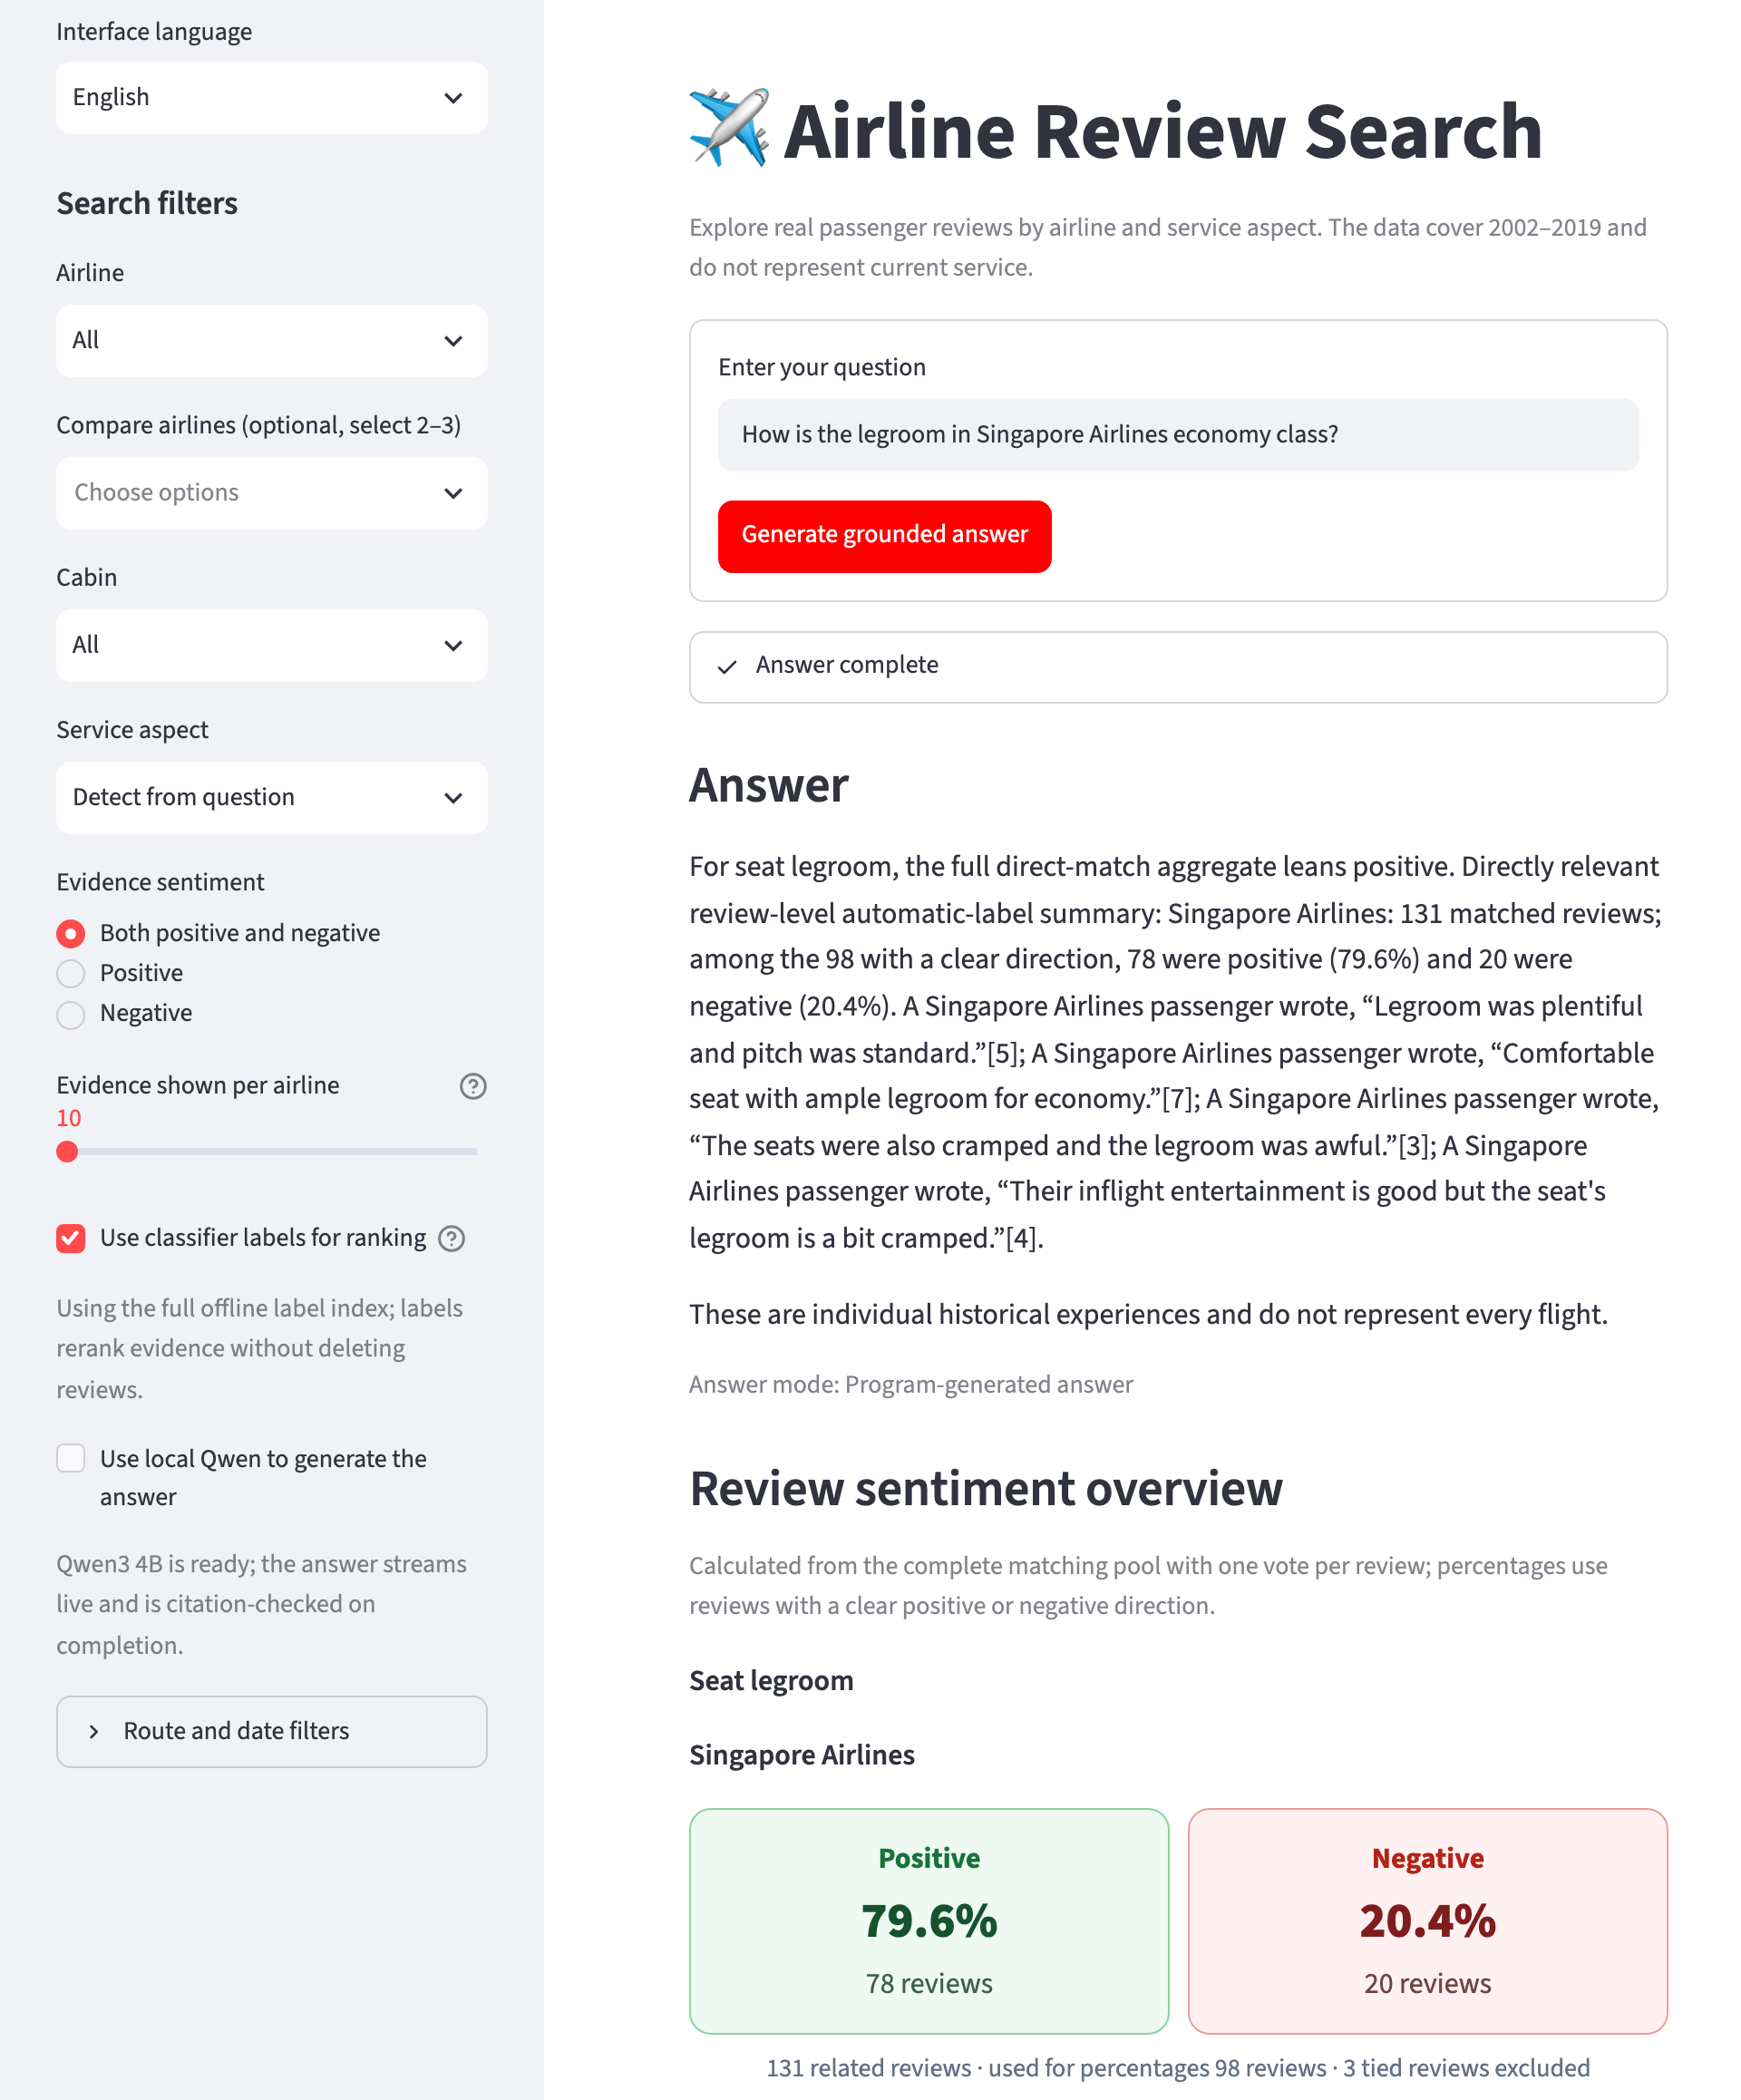
\includegraphics[width=0.86\textwidth]{figures/ui_single.png}
\caption{The interface, single-airline question in English mode. The parser detected airline, aspect (seat) and
sub-attribute (legroom). The program-written answer cites four sentences; the overview counts 131 matching reviews, 98
of them with a clear direction (79.6\% positive).}
\label{fig:ui}
\end{figure*}

\begin{figure*}[t]
\centering
\begin{subfigure}[t]{0.44\textwidth}
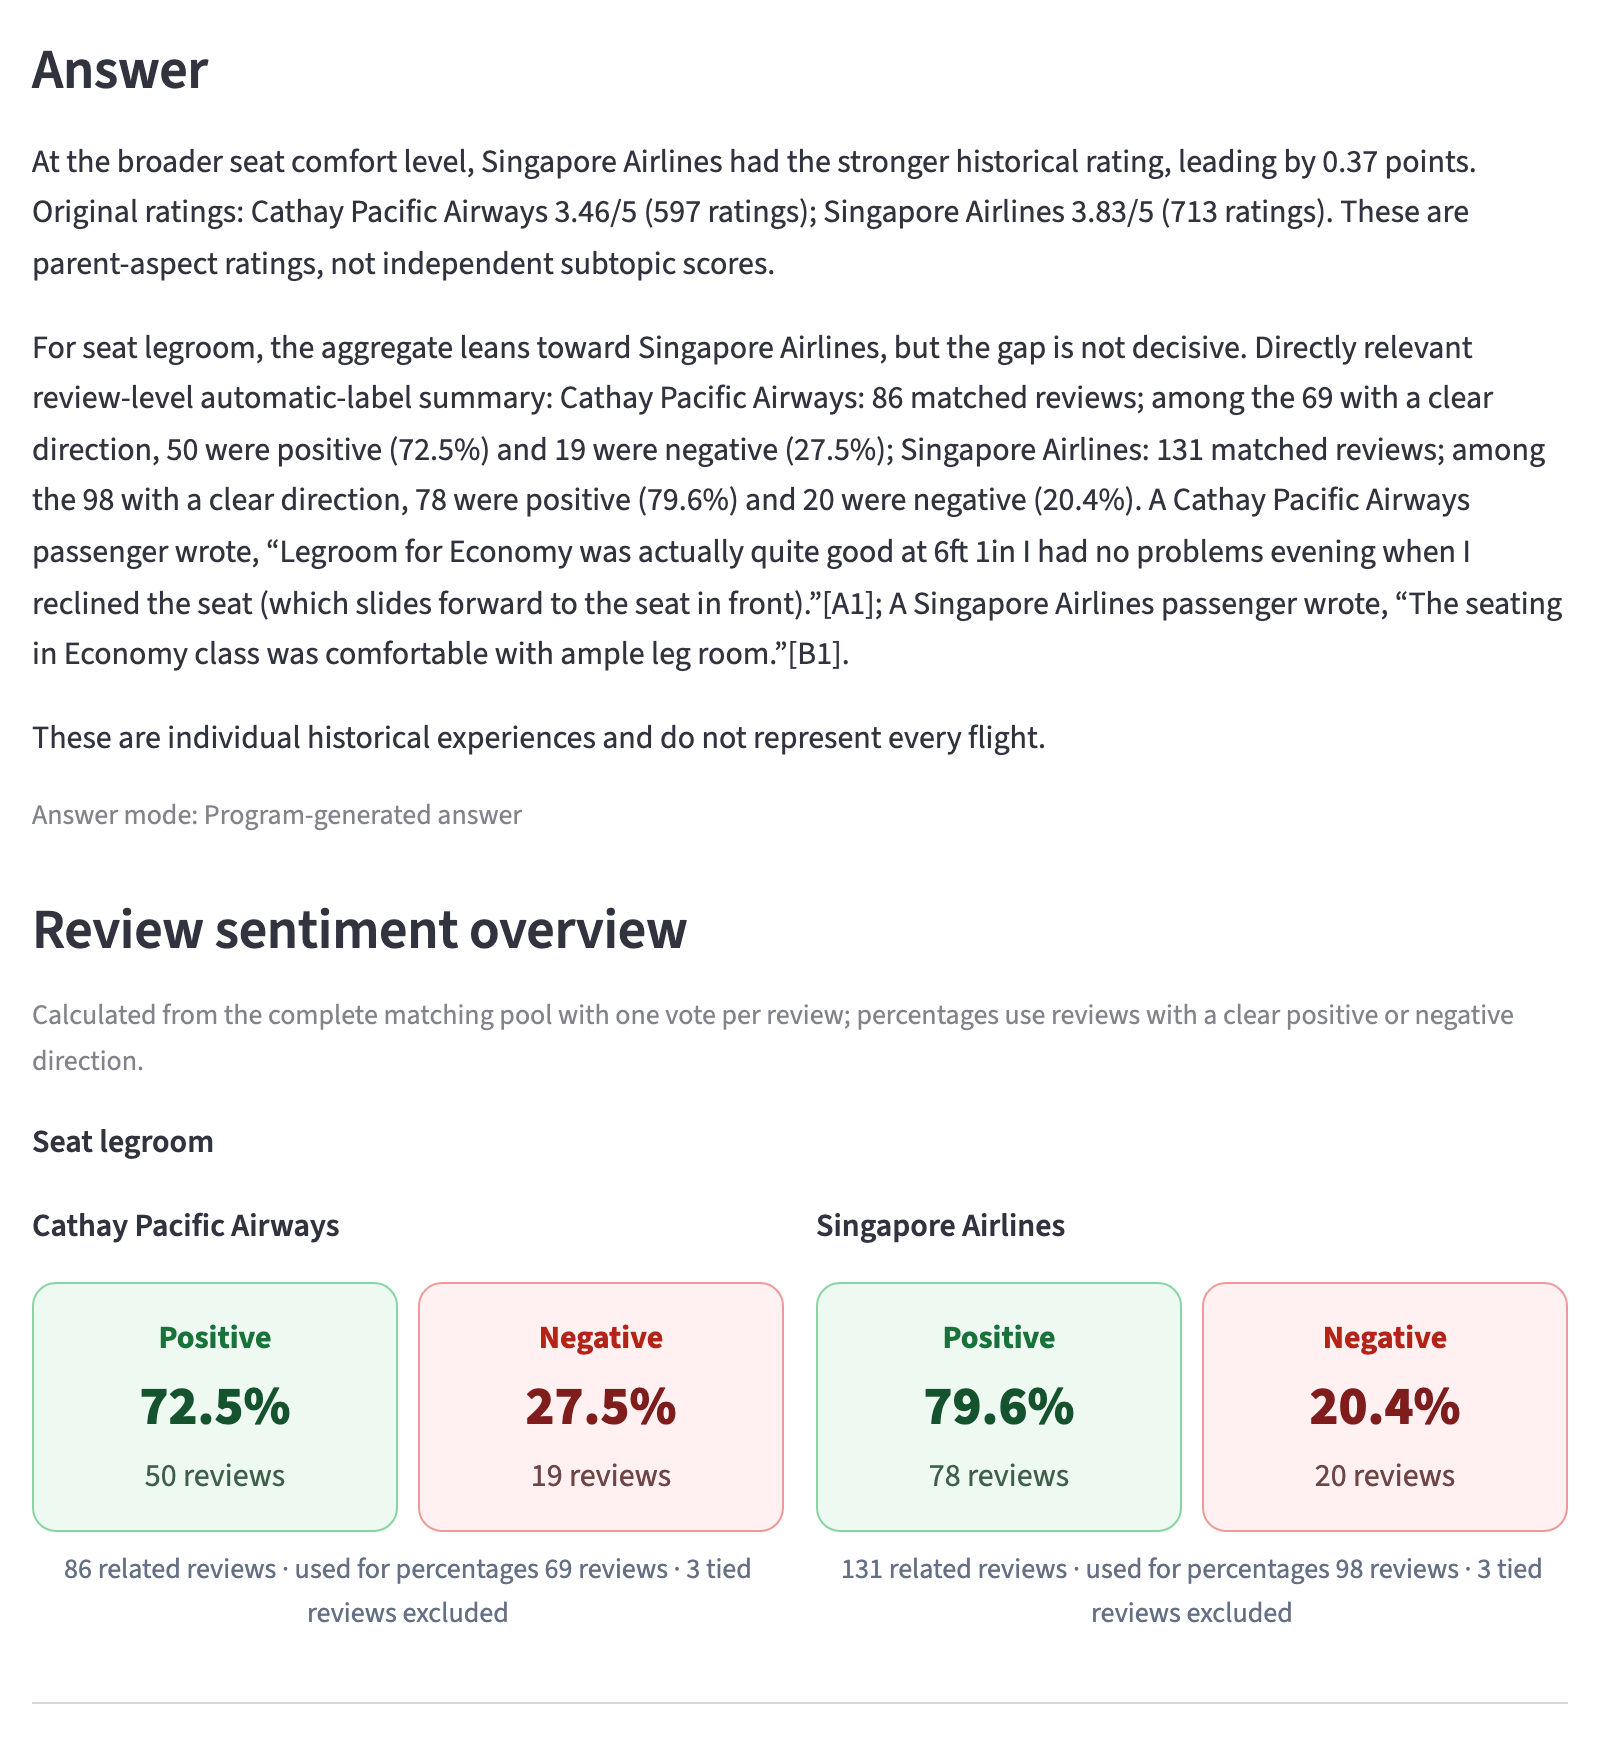
\includegraphics[height=78mm]{figures/ui_compare_answer.png}
\caption{Answer, full-pool tally and rating test.}
\end{subfigure}\hfill
\begin{subfigure}[t]{0.55\textwidth}
\raggedleft
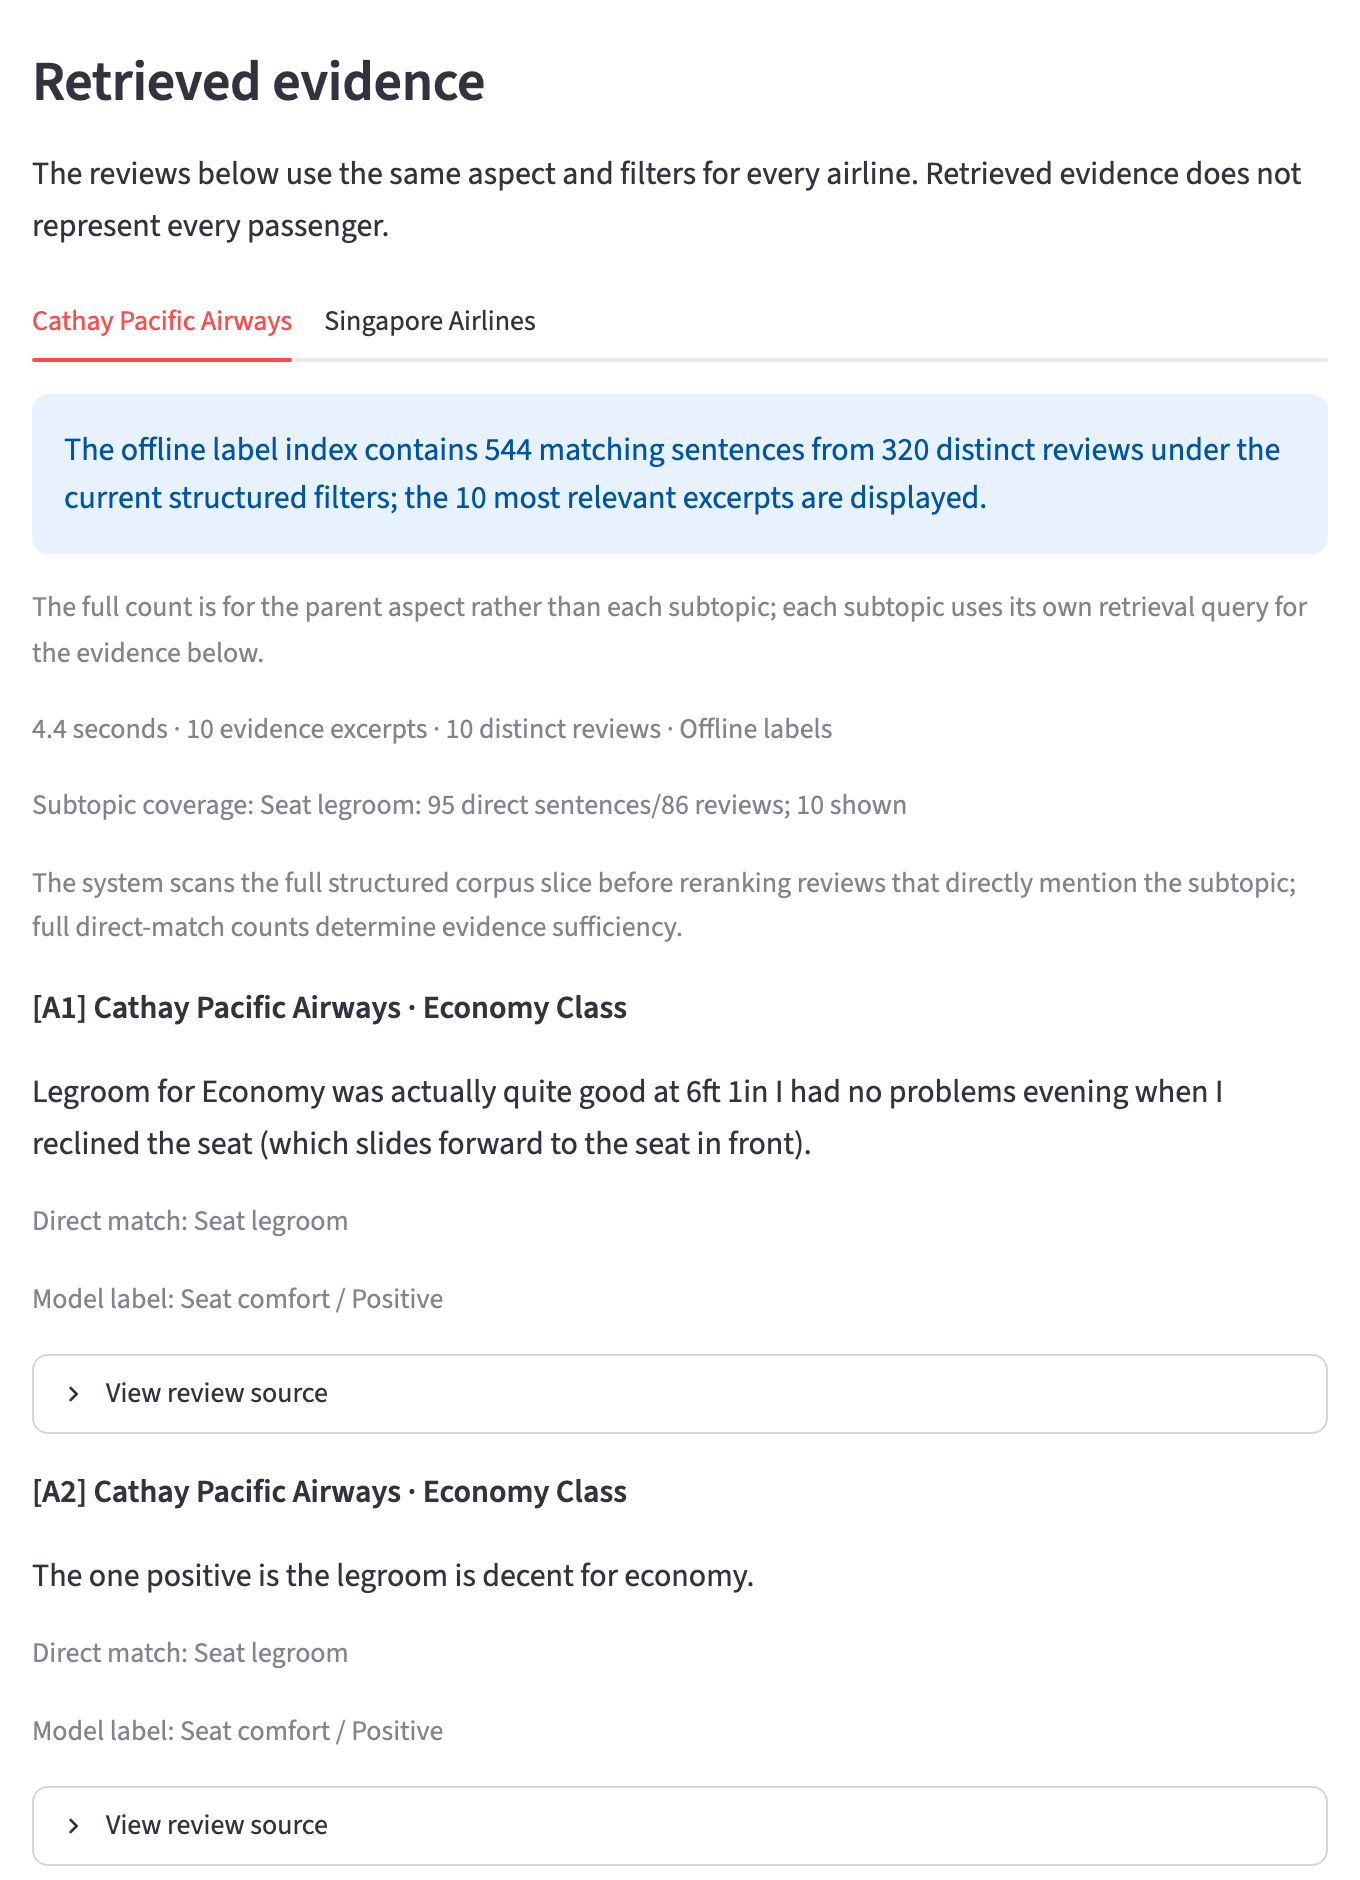
\includegraphics[height=78mm]{figures/ui_compare_evidence.png}
\caption{Evidence tab with coverage counts.}
\end{subfigure}
\caption{Comparison of Cathay Pacific and Singapore Airlines on economy legroom. Singapore Airlines' higher
seat-comfort rating (3.83 vs.\ 3.46 of 5) is significant and reported for the parent aspect; the legroom tallies (72.5\%
vs.\ 79.6\% positive) are reported as not decisive. The evidence tab shows 95 direct legroom sentences in 86 reviews and
a retrieval time of 4.5\,s (a separate run from \cref{tab:five}).}
\label{fig:ui-compare}
\end{figure*}

%--------------------------------------------------------------- Experiments
\section{Experiments}
\label{sec:exp}

\subsection{Setup and evaluation data}
\label{sec:data}

E1--E5 and E8 run on an Apple M1 Pro (16\,GB); E6 and E7 ran on a Linux machine with an AMD Radeon RX 7800 XT.
Intervals are 95\% bootstrap intervals at the query, question or parent-review level (\num{10000} resamples for E1 and
E5, \num{2000} for E4, E6 and E7). The evaluation data are: 30 airline $\times$ sub-attribute retrieval units
(E1); 20 fixed end-to-end questions written in Chinese (12 single-airline, 5 comparisons, 3 multi-aspect; E2, E5);
a \num{1000}-sentence human-labelled gold set (E3, E4); 20 English single-attribute questions for the factorial
ablation (E6, Appendix~\ref{app:factorial}); and held-out passenger ratings for the airline ranking (E7).

\paragraph{Gold set (Q4).} Candidates came from \num{478969} sentences after removing route lines, duplicates, sentences
under five words and reviews without an overall score. We sampled half from reviews scoring $\ge$7 and half from
$\le$4, about 120 per rated aspect, plus sentences with no clear aspect, and shuffled them. Three annotators labelled
every sentence independently seeing \emph{only the sentence}: airline and ratings were hidden because ratings are also
the weak-label source. A written guideline fixed edge cases such as mixed sentiment. On the frozen \num{1000} sentences, agreement exceeds
80\% on all three tasks (\cref{tab:agree}); subjectivity has moderate Fleiss' $\kappa$~\cite{fleiss} because only 8\% of
sentences are objective. Across all \num{1100} labelled sentences, the two tasks the brief requires, subjectivity and
polarity, still exceed 80\%, but aspect agreement is 75.2\%: the 100 sentences left out include 15 that the guideline
drops as unclear and 52 on which the three annotators chose three different aspects. Disagreements were resolved by majority vote, then by AI-assisted adjudication confirmed one by one by a
human reviewer, who changed 9 sentences. Sampling balanced the review scores (502 vs.\ 498 sentences) but not the labels: 143 sentences from high-scoring reviews
are complaints, while only 49 from low-scoring reviews are praise. We kept this natural skew rather than resample after
labelling, and report macro and per-class scores. The set has 548 negative, 371 positive and 81 objective sentences, no
duplicate texts, and is stored as \nolinkurl{data/eval/eval.xls} in standard benchmark format (Appendix~\ref{app:eval}).

\begin{table}[t]
\centering\small
\caption{Pairwise agreement of the three original annotators. Frozen: the \num{1000} gold sentences (\num{3000}
pairs), with Fleiss' $\kappa$. All: every labelled sentence (\num{1100}; \num{3300} pairs).}
\label{tab:agree}
\setlength{\tabcolsep}{4pt}
\begin{tabular}{@{}lrrrr@{}}
\toprule
\textbf{Field} & \textbf{Agreeing} & \textbf{Frozen} & \textbf{$\kappa$} & \textbf{All} \\
\midrule
Subjectivity & \num{2783} & 92.8\% & 0.572 & 90.9\% \\
Polarity (incl.\ NA) & \num{2730} & 91.0\% & 0.841 & 89.3\% \\
Aspect (8 classes) & \num{2426} & 80.9\% & 0.778 & 75.2\% \\
All three at once & \num{2250} & 75.0\% & 0.732 & 69.8\% \\
\bottomrule
\end{tabular}
\end{table}

\paragraph{Scope of the gold set.} We labelled \num{1100} sentences and froze \num{1000}, chosen \emph{after} labelling
by keeping sentences whose original aspect labels agreed; agreement on the frozen set is therefore higher than on
all labelled sentences (\cref{tab:agree}). Some earlier classifier variants were also scored on these sentences during
development. We treat the set as a well-adjudicated benchmark rather than a pristine test set; for the distilled model
(E4), selection never read it and it was scored exactly once.

\subsection{E1: Does hybrid retrieval rank better? (Q3)}
\label{sec:exp-ret}

\paragraph{Protocol.} Each of the 30 units (e.g.\ \emph{Singapore Airlines, legroom}) uses the same metadata constraints
for every configuration. Relevance is graded automatically: a sentence that explicitly names the sub-attribute is highly
relevant; one the classifier labels as the same aspect and subjective is partially relevant. We report P@5, Recall@50,
MRR, NDCG@10~\cite{ndcg} and Success@10.

\begin{table*}[t]
\centering\small
\caption{E1: retrieval quality on 30 airline $\times$ sub-attribute queries (automatic graded relevance). Best per column
in bold; latency is the warm median per query including metadata filtering. These are the retriever configurations; the
deployed pipeline also scans the filtered slice for sub-attribute mentions (\cref{sec:ret}).}
\label{tab:retrieval}
\begin{tabular}{@{}lrrrrrr@{}}
\toprule
\textbf{Configuration} & \textbf{P@5} & \textbf{Recall@50} & \textbf{MRR} & \textbf{NDCG@10} & \textbf{Success@10} & \textbf{Latency} \\
\midrule
BM25 & \best{0.880} & \best{0.403} & 0.950 & 0.790 & 1.000 & 0.534\,s \\
Dense (MiniLM) & 0.753 & 0.307 & 0.867 & 0.686 & 1.000 & \best{0.057\,s} \\
\rowcolor{shade} Hybrid + RRF (default) & \best{0.880} & 0.381 & \best{0.961} & \best{0.810} & 1.000 & 0.592\,s \\
Hybrid + RRF + cross-encoder & 0.827 & 0.387 & 0.933 & 0.744 & 1.000 & 0.714\,s \\
\bottomrule
\end{tabular}
\end{table*}

\begin{figure}[t]
\centering
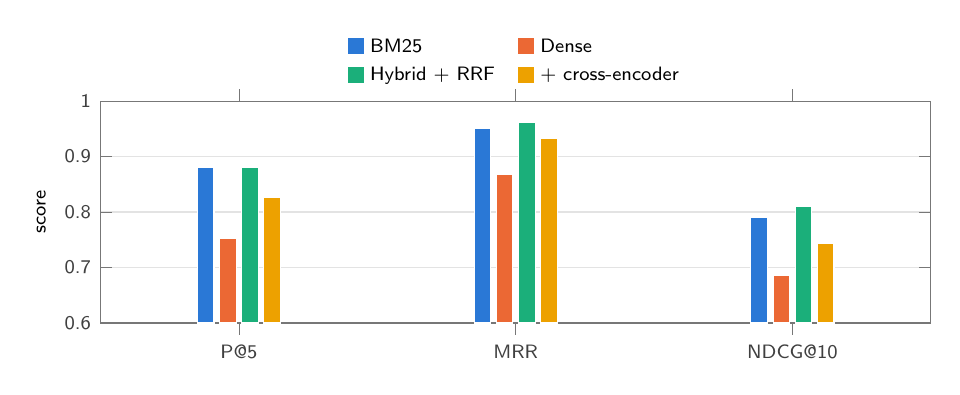
\begin{tikzpicture}
\begin{axis}[paper, ybar, width=\columnwidth, height=44mm, barlegend, bar width=6pt, ymin=0.6, ymax=1.0,
  symbolic x coords={P@5,MRR,NDCG@10}, xtick=data, enlarge x limits=0.25, ylabel={score},
  legend style={at={(0.5,1.02)},anchor=south, legend columns=2}]
\addplot[fill=s1, draw=white] coordinates {(P@5,0.880) (MRR,0.950) (NDCG@10,0.790)};
\addplot[fill=s2, draw=white] coordinates {(P@5,0.753) (MRR,0.867) (NDCG@10,0.686)};
\addplot[fill=s3, draw=white] coordinates {(P@5,0.880) (MRR,0.961) (NDCG@10,0.810)};
\addplot[fill=s4, draw=white] coordinates {(P@5,0.827) (MRR,0.933) (NDCG@10,0.744)};
\legend{BM25, Dense, Hybrid + RRF, + cross-encoder}
\end{axis}
\end{tikzpicture}
\caption{E1: precision-oriented metrics from \cref{tab:retrieval} (axis starts at 0.6).}
\label{fig:retrieval}
\end{figure}

\paragraph{Results.} Hybrid + RRF ranks best on MRR and NDCG@10 and ties BM25 on P@5 (\cref{tab:retrieval,fig:retrieval}).
Dense retrieval alone is weakest: it ranks topically related but off-attribute sentences high; fusion keeps BM25's
precision and adds paraphrases further down. The gain over BM25 is not significant with 30 queries
($\Delta$NDCG@10 $=+0.020$, CI $[-0.036,+0.073]$). The cross-encoder \emph{hurts} ($\Delta$NDCG@10 $=-0.066$, CI
$[-0.114,-0.019]$): trained on MS MARCO web questions, it prefers sentences that answer a question in general, such as
a long comfort description, over short sentences that name the attribute. We therefore use it only to order candidates
that already mention the requested sub-attribute. Success@10 is 1.0 everywhere, so differences are about ordering and
coverage. These relevance labels are reproducible but favour explicit mentions, which advantages BM25 and under-counts dense
paraphrases (``knees touching the seat in front''); human judgements would make the comparison stronger.

\subsection{E2: How fast is a query? (Q2)}
\label{sec:exp-speed}

\Cref{tab:five} reports five of the 20 evaluation questions, chosen to cover the supported query types, as warm runs
with the local model on. \emph{Retrieval} covers parsing, filtering, BM25, dense search, fusion, reranking and evidence
selection; \emph{first token} is measured from submission; \emph{total} runs until the checked answer is shown.
\Cref{fig:latency} shows that retrieval is a small share of the wait: the 4B model on a laptop dominates, which we
mitigate by streaming. Timed alone over the full pool without filters (the 30 E1 queries, warm medians), BM25 top-20 takes 503\,ms, FAISS
top-20 20\,ms, hybrid retrieval (both top-100 lists and RRF) 519\,ms and cross-encoder reranking of 100 candidates
108\,ms (\nolinkurl{experiments/final_auto_eval/component_latency.py}); scoring all sentences with BM25 dominates. With the LLM off, the
program-written path averaged 5.0\,s per question over a 40-question smoke test.

\begin{table}[t]
\centering\small
\caption{E2: five representative queries (asked in Chinese; original wording and results in Appendix~\ref{app:queries}).
Answer: model draft (D), repaired draft (R) or program-written (P). The All-20 rows include the cold first question.}
\label{tab:five}
\setlength{\tabcolsep}{3.5pt}
\begin{tabularx}{\columnwidth}{@{}lYrrrc@{}}
\toprule
& \textbf{Query} & \textbf{Retr.} & \textbf{1st tok.} & \textbf{Total} & \textbf{Ans.} \\
\midrule
Q05 & Emirates economy: refunds and rebooking? & 2.2\,s & 23.8\,s & 26.8\,s & D \\
Q10 & Qatar business: film selection? & 2.2\,s & 18.4\,s & 33.6\,s & R \\
Q24 & Cathay vs.\ SIA economy legroom? & 5.1\,s & 28.4\,s & 57.8\,s & R \\
Q28 & SIA economy: legroom, recline, comfort, cleanliness? & 9.7\,s & 27.4\,s & 53.6\,s & P \\
Q30 & SIA economy: food, value, ground service? & 6.9\,s & 50.8\,s & 82.0\,s & P \\
\midrule
\multicolumn{2}{@{}l}{\textit{All 20: median}} & 2.9\,s & 24.3\,s & 40.8\,s & \\
\multicolumn{2}{@{}l}{\textit{All 20: P95}} & 10.5\,s & 41.9\,s & 72.3\,s & \\
\bottomrule
\end{tabularx}
\end{table}

\begin{figure}[t]
\centering
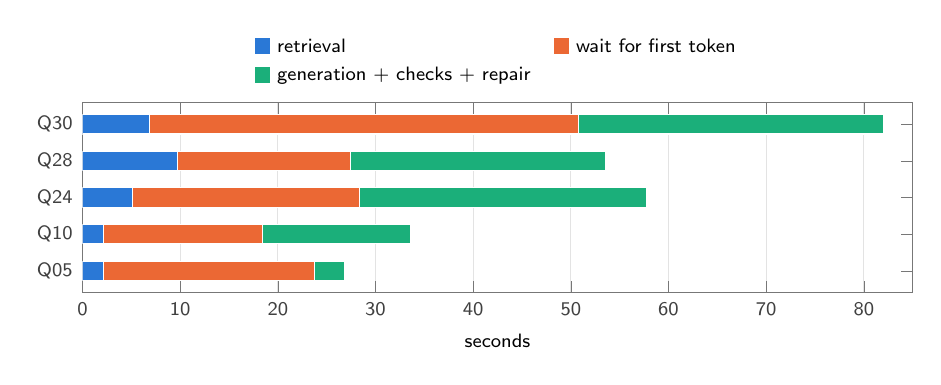
\begin{tikzpicture}
\begin{axis}[paper, xbar stacked, width=\columnwidth, height=40mm, barlegend, bar width=7pt,
  xmin=0, xmax=85, xlabel={seconds}, ymajorgrids=false, xmajorgrids,
  symbolic y coords={Q30,Q28,Q24,Q10,Q05}, ytick=data, y dir=reverse,
  legend style={at={(0.5,1.03)},anchor=south, legend columns=2}, enlarge y limits=0.15]
\addplot[fill=s1, draw=white] coordinates {(2.2,Q05) (2.2,Q10) (5.1,Q24) (9.7,Q28) (6.9,Q30)};
\addplot[fill=s2, draw=white] coordinates {(21.6,Q05) (16.2,Q10) (23.3,Q24) (17.7,Q28) (43.9,Q30)};
\addplot[fill=s3, draw=white] coordinates {(3.0,Q05) (15.2,Q10) (29.4,Q24) (26.2,Q28) (31.2,Q30)};
\legend{retrieval, wait for first token, generation + checks + repair}
\end{axis}
\end{tikzpicture}
\caption{E2: where the time goes for the queries in \cref{tab:five}.}
\label{fig:latency}
\end{figure}

\subsection{E3: How good is the classifier? (Q4)}
\label{sec:exp-cls}

\Cref{tab:cls} gives the summary metrics used for model selection (macro-F1 over aspects and polarities on the 919
subjective sentences, joint accuracy, recall of each subjectivity class); \cref{tab:prf} gives per-class precision,
recall and F1 as the brief requests, and \cref{fig:aspect} breaks aspect F1 down by class.

\begin{table}[t]
\centering\small
\caption{E3: classifier quality on the gold set (\%). Aspect and polarity F1 are macro-averaged over 919 subjective
sentences. Shaded: the distilled student, selected to replace v4.1 (\cref{sec:exp-distill}). Joint: aspect and polarity both
correct; S-rec./O-rec.: recall of subjective/objective sentences over all \num{1000}. v4.1 is the weak-supervision
classifier the interface uses; r36 is the LLM teacher (\cref{tab:approach}); targets were fixed at the project start.}
\label{tab:cls}
\setlength{\tabcolsep}{3pt}
\begin{tabularx}{\columnwidth}{@{}Yrrrrr@{}}
\toprule
\textbf{Model} & \textbf{Asp.} & \textbf{Pol.} & \textbf{Joint} & \textbf{S-rec.} & \textbf{O-rec.} \\
\midrule
v4.1: TF-IDF + rules (weak) & 61.1 & 82.1 & 56.1 & 99.9 & 7.4 \\
TF-IDF + MiniLM (weak) & 68.1 & 85.2 & 61.5 & \best{100.0} & 21.0 \\
\rowcolor{shade} Distilled (weak + teacher) & 70.4 & 86.2 & 63.5 & 96.8 & 66.7 \\
r36 LLM teacher & \best{74.1} & \best{91.8} & \best{70.8} & 96.8 & \best{76.5} \\
\midrule
\textit{Project target} & 85 & 90 & 80 & 97 & -- \\
\bottomrule
\end{tabularx}
\end{table}

\begin{table*}[t]
\centering\small
\caption{E3: precision / recall / F1 (\%) per class. The three-class label is the \texttt{label} column of eval.xls.
Polarity is computed on the 919 gold-subjective sentences, where a wrong ``objective'' prediction counts as a miss.}
\label{tab:prf}
\begin{tabular}{@{}l*{3}{rrr}@{}}
\toprule
 & \multicolumn{3}{c}{\textbf{v4.1 (previous)}} & \multicolumn{3}{c}{\textbf{Distilled student}} & \multicolumn{3}{c}{\textbf{r36 teacher}} \\
\cmidrule(lr){2-4}\cmidrule(lr){5-7}\cmidrule(l){8-10}
\textbf{Class} & P & R & F1 & P & R & F1 & P & R & F1 \\
\midrule
\multicolumn{10}{@{}l}{\textit{Three-class label}} \\
\quad negative & 76.8 & 88.3 & 82.2 & 87.9 & 87.4 & 87.6 & 91.4 & 93.4 & 92.4 \\
\quad positive & 76.6 & 74.9 & 75.7 & 82.0 & 82.2 & 82.1 & 92.0 & 86.5 & 89.2 \\
\quad objective & 85.7 & 7.4 & 13.6 & 65.1 & 66.7 & 65.9 & 68.1 & 76.5 & 72.1 \\
\quad macro average & 79.7 & 56.9 & 57.2 & 78.3 & 78.8 & \best{78.5} & 83.8 & 85.5 & 84.6 \\
\quad accuracy & \multicolumn{3}{r}{76.8} & \multicolumn{3}{r}{\best{83.8}} & \multicolumn{3}{r}{89.5} \\
\midrule
\multicolumn{10}{@{}l}{\textit{Subjectivity detection}} \\
\quad subjective & 92.4 & 99.9 & 96.0 & 97.1 & 96.8 & 96.9 & 97.9 & 96.8 & 97.4 \\
\quad objective & 85.7 & 7.4 & 13.6 & 65.1 & 66.7 & 65.9 & 68.1 & 76.5 & 72.1 \\
\midrule
\multicolumn{10}{@{}l}{\textit{Polarity detection (gold-subjective sentences)}} \\
\quad negative & 83.9 & 88.3 & 86.0 & 89.9 & 87.4 & 88.6 & 93.3 & 93.4 & 93.3 \\
\quad positive & 81.5 & 74.9 & 78.1 & 85.4 & 82.2 & 83.8 & 94.1 & 86.5 & 90.2 \\
\bottomrule
\end{tabular}
\end{table*}

\begin{figure}[t]
\centering
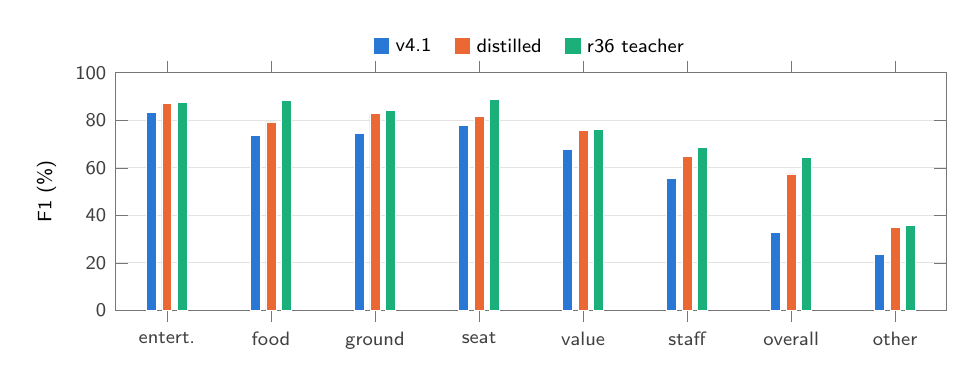
\begin{tikzpicture}
\begin{axis}[paper, ybar, width=\columnwidth, height=46mm, barlegend, bar width=3.6pt, ymin=0, ymax=100,
  symbolic x coords={entert.,food,ground,seat,value,staff,overall,other},
  xtick=data, enlarge x limits=0.07, ylabel={F1 (\%)}, legend style={at={(0.5,1.02)},anchor=south}]
\addplot[fill=s1, draw=white, line width=0.3pt] coordinates {(entert.,83.1) (food,73.7) (ground,74.3) (seat,77.9) (value,67.8) (staff,55.7) (overall,32.9) (other,23.4)};
\addplot[fill=s2, draw=white, line width=0.3pt] coordinates {(entert.,86.9) (food,79.3) (ground,82.8) (seat,81.7) (value,75.6) (staff,64.8) (overall,57.4) (other,35.0)};
\addplot[fill=s3, draw=white, line width=0.3pt] coordinates {(entert.,87.3) (food,88.2) (ground,84.2) (seat,88.6) (value,76.3) (staff,68.6) (overall,64.3) (other,35.7)};
\legend{v4.1, distilled, r36 teacher}
\end{axis}
\end{tikzpicture}
\caption{E3: aspect F1 per class on subjective gold sentences (supports: entertainment 115, food 99, ground 238, seat 86,
value 130, staff 103, overall 101, other 47). Concrete aspects are easy; \emph{overall} and \emph{other} are hard for
every model.}
\label{fig:aspect}
\end{figure}

\paragraph{Results.} Objective sentences are the main weakness of weak supervision: with 179 objective training
examples, v4.1 finds 7.4\% of them and the embedding model 21.0\%; teacher labels raise this to 66.7\% at a cost of 3
points of subjective recall, and three-class macro-F1 rises from 57.2 to 78.5. Aspect errors are concentrated: the
student's most frequent confusions are \emph{staff} predicted as \emph{food} (18 sentences, mostly crew handling of the
meal service, e.g.\ ``No refills of drinks offered during or after the meal''), \emph{ground} as \emph{value} (16,
mostly refunds and compensation) and \emph{overall} vs.\ \emph{other}. These sentences genuinely concern two aspects,
so part of the gap to the 85\% target reflects the single-aspect label definition. No model, not even the LLM teacher,
reaches every target; we report this rather than tune on the gold set.

\subsection{E4: Can a fast classifier inherit the LLM's labels? (Q5)}
\label{sec:exp-distill}

\paragraph{Motivation.} The label index drives the tally users see. Built with v4.1 it marked only 0.6\% of the corpus
objective, against 8.1\% in gold, so almost every factual sentence was counted as an opinion. The teacher is far better
but would need about three days for the corpus.

\paragraph{Protocol.} (i)~We drew \num{10003} sentences from \num{1154} parent reviews in the \emph{development} split of
the weak labels, excluding every gold sentence, its parent review and its normalised text, and any text seen in
weak-label training. (ii)~The teacher labelled all of them in 89 minutes with no invalid outputs (12.8\% objective).
(iii)~We split by parent review into pseudo-train (\num{7355}) and pseudo-dev (\num{2648}). (iv)~Before training we fixed
three students with identical features that differ only in supervision: \emph{weak} (weak labels only, reproducing a
teammate's model), \emph{teacher} (teacher labels only) and \emph{mixed} (both, teacher examples up-weighted so each
source carries equal weight). (v)~The winner was selected by a fixed rank score against the \emph{teacher} on
pseudo-dev ($0.35\,$aspect F1 $+\,0.20\,$polarity F1 $+\,0.35\,$joint $+\,0.10\,$subjective recall, minus penalties
when subjective recall falls below 97\% or objective recall below 60\%); a file-read guard prevented access to gold. (vi)~Also fixed in advance: the winner replaces v4.1 only if it
beats v4.1 on gold in both rank score and joint accuracy.

\begin{table*}[t]
\centering\small
\caption{E4: supervision ablation. Left: agreement with the teacher on pseudo-dev (used for selection). Right: the same
models on human gold, scored once after selection. Features are identical; only the training labels differ.}
\label{tab:distill}
\begin{tabular}{@{}lrrr@{\hspace{8mm}}rrrr@{}}
\toprule
 & \multicolumn{3}{c}{\textbf{vs.\ teacher, pseudo-dev}} & \multicolumn{4}{c}{\textbf{vs.\ human gold}} \\
\cmidrule(r{8mm}){2-4}\cmidrule(l){5-8}
\textbf{Supervision} & \textbf{Joint} & \textbf{Obj.\ rec.} & \textbf{Rank} & \textbf{Aspect F1} & \textbf{Joint} & \textbf{Obj.\ rec.} & \textbf{Rank} \\
\midrule
v4.1 production (reference) & 54.0 & 3.9 & 0.637 & 61.1 & 56.1 & 7.4 & 0.648 \\
Weak only & 59.9 & 18.9 & 0.692 & 68.1 & 61.5 & 21.0 & 0.705 \\
Teacher only (7.4k) & 64.0 & \best{75.7} & 0.662 & \best{71.4} & 61.4 & \best{76.5} & 0.651 \\
\rowcolor{shade} Weak + teacher (selected) & \best{65.8} & 67.1 & \best{0.729} & 70.4 & \best{63.5} & 66.7 & \best{0.735} \\
\bottomrule
\end{tabular}
\end{table*}

\begin{figure}[t]
\centering
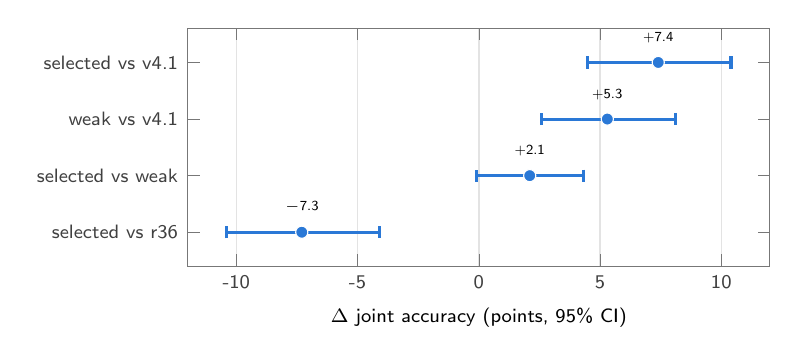
\begin{tikzpicture}
\begin{axis}[paper, width=0.74\columnwidth, height=46mm,
  xmin=-12, xmax=12, ymin=0.4, ymax=4.6, ytick={1,2,3,4}, y dir=reverse,
  yticklabels={selected vs v4.1, weak vs v4.1, selected vs weak, selected vs r36},
  ymajorgrids=false, xmajorgrids, xlabel={$\Delta$ joint accuracy (points, 95\% CI)},
  extra x ticks={0}, extra x tick labels={}, extra x tick style={grid style={draw=black, line width=0.6pt}}]
\addplot[only marks, mark=*, mark size=2.2pt, color=s1, mark options={draw=white},
  error bars/.cd, x dir=both, x explicit, error bar style={draw=s1, line width=1.1pt}, error mark options={draw=s1, line width=1.1pt, mark size=2.2pt, rotate=90}]
  coordinates {(7.4,1) -= (2.9,0) += (3.0,0)  (5.3,2) -= (2.7,0) += (2.8,0)  (2.1,3) -= (2.2,0) += (2.2,0)  (-7.3,4) -= (3.1,0) += (3.2,0)};
\node[font=\sffamily\tiny, anchor=south] at (axis cs:7.4,1) [yshift=3.5pt] {+7.4};
\node[font=\sffamily\tiny, anchor=south] at (axis cs:5.3,2) [yshift=3.5pt] {+5.3};
\node[font=\sffamily\tiny, anchor=south] at (axis cs:2.1,3) [yshift=3.5pt] {+2.1};
\node[font=\sffamily\tiny, anchor=south] at (axis cs:-7.3,4) [yshift=3.5pt] {$-$7.3};
\end{axis}
\end{tikzpicture}
\caption{E4: paired differences in joint accuracy on gold (parent-review bootstrap). CIs: $[+4.5,+10.4]$,
$[+2.6,+8.1]$, $[-0.1,+4.3]$, $[-10.4,-4.1]$.}
\label{fig:distill}
\end{figure}

\paragraph{Results.} The mixed student was selected on pseudo-dev and passed the adoption rule on gold
(\cref{tab:distill}). Replacing the v4.1 features by TF-IDF + MiniLM gives +5.3 points of joint accuracy (confounded by
v4.1's rule layer); adding teacher labels gives a further +2.1, not significant at the 95\% level (CI $[-0.1,+4.3]$, \cref{fig:distill}), and lifts
objective recall from 21.0\% to 66.7\%. Teacher labels are valuable per example: the teacher-only student, trained on
7.4k sentences, has the best aspect F1 and objective recall of the three, but is weaker on polarity than models that also
see the \num{231779} weak labels, so mixing works best overall. Rebuilding the \num{529031}-label index takes 18\,s
instead of an estimated three days; the corpus's objective share goes from 0.6\% to 13.0\% (teacher: 12.8\% on the
sample), and 32\% of aspect and 24\% of polarity labels change. The student remains 7.3 points below its teacher.

\paragraph{Status.} Because a third of the labels change, the interface switches to the new index only after the
downstream statistics are re-run; E5 and E6 below were produced with the v4.1 labels, and E7 uses a separate
diagnostic classifier (TF-IDF and logistic regression).

\subsection{E5: Are the answers grounded? (Q4)}
\label{sec:exp-rag}

We evaluate the whole system on the 20 questions with RAGAS-style metrics~\cite{ragas}: \emph{faithfulness} (share of
answer claims supported by evidence), \emph{answer relevance} and \emph{context precision} (share of displayed evidence
relevant to the question). The judge is the local Qwen3-4B with a fixed rubric; it sees the displayed evidence and the
program-computed ratings and tallies, so correct aggregate numbers are not marked unsupported.

\begin{table}[t]
\centering\small
\caption{E5: answer-level metrics of the guarded system (20 questions).}
\label{tab:rag}
\begin{tabular}{@{}lrl@{}}
\toprule
\textbf{Metric} & \textbf{Score} & \textbf{95\% CI} \\
\midrule
Faithfulness & 0.843 & [0.800, 0.890] \\
Answer relevance & 0.988 & [0.963, 1.000] \\
Context precision & 0.600 & [0.517, 0.681] \\
\bottomrule
\end{tabular}
\end{table}

\paragraph{Results.} Answers stay on topic and are mostly grounded (\cref{tab:rag}). Context precision is the weakest:
about 40\% of displayed sentences were judged not directly relevant, partly because we deliberately show a
counter-example and broader-aspect context (E6). The scores describe the \emph{system}: the model's first draft was used
for 1 question, its repair for 3 and the program-written answer for 16, because the 4B model's drafts often failed the
strict citation or number checks. Since generator and judge are the same model, these are reproducible automatic
proxies, not independent human scores.

\subsection{E6: What does each answer-side component buy? (Q5)}
\label{sec:exp-abl}

The brief asks for the gain of each innovation alone and in combination. We therefore ran a full $2^3$ factorial
ablation of the three factors of \cref{sec:gen}: X (full-pool statistics), Y (balanced, label-consistent examples) and
Z (validation, one repair, program-written fallback).

\paragraph{Protocol.} We use 20 English single-airline, single-attribute questions from the development smoke set
(Appendix~\ref{app:factorial}), fixed before scoring. Each question has a frozen pool of up to 30 candidates ranked
without labels; all eight configurations share the pool, the prompt and a budget of four citations. With X off,
corpus counts and the overall direction are hidden from generation, validation and fallback; with Y off, the top four
candidates are used; with Z off, the model's draft is returned unchecked. Qwen3-4B-Instruct-2507 (BF16, Transformers
backend on an AMD Radeon RX 7800 XT) both generates and judges, using the metrics of E5 with answer relevance scored
0--4 and rescaled. Each question gets one draft per X/Y setting, shared by its Z-off and Z-on variants, so the run produced 80 drafts,
54 repair attempts and 160 final answers. Intervals come from 2,000
paired bootstrap resamples over questions (seed 6127), without multiple-comparison adjustment.

\begin{table*}[t]
\centering\small
\caption{E6: factorial ablation (20 questions per configuration). Code XYZ, 1 = component on. $\Delta$: paired difference
in faithfulness against the baseline, with 95\% bootstrap interval.}
\label{tab:factorial}
\begin{tabular}{@{}llrlrr@{}}
\toprule
\textbf{Code} & \textbf{Configuration} & \textbf{Faithfulness} & \textbf{$\Delta$ vs.\ baseline [95\% CI]} & \textbf{Answer rel.} & \textbf{Context prec.} \\
\midrule
000 & Baseline & 0.887 & -- & \best{1.000} & 0.808 \\
100 & X only & 0.860 & $-0.028$ [$-0.078$, $+0.024$] & 0.988 & 0.808 \\
010 & Y only & 0.918 & $+0.031$ [$-0.029$, $+0.088$] & \best{1.000} & \best{0.871} \\
001 & Z only & 0.917 & $+0.030$ [$+0.003$, $+0.063$] & \best{1.000} & 0.808 \\
110 & X + Y & 0.902 & $+0.014$ [$-0.031$, $+0.061$] & \best{1.000} & 0.854 \\
101 & X + Z & 0.868 & $-0.020$ [$-0.080$, $+0.039$] & 0.925 & 0.808 \\
\rowcolor{shade} 011 & Y + Z & \best{0.940} & $+0.053$ [$+0.004$, $+0.106$] & 0.975 & \best{0.871} \\
111 & X + Y + Z (deployed) & 0.885 & $-0.002$ [$-0.074$, $+0.065$] & 0.975 & 0.854 \\
\bottomrule
\end{tabular}
\end{table*}

\begin{figure}[t]
\centering
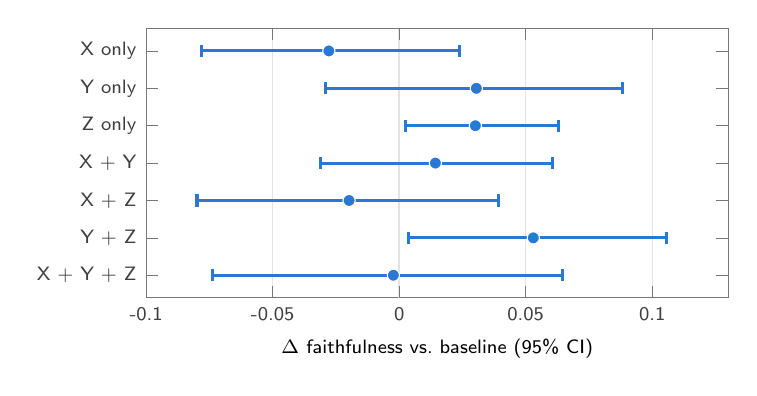
\begin{tikzpicture}
\begin{axis}[paper, width=0.74\columnwidth, height=50mm,
  xmin=-0.1, xmax=0.13, ymin=0.4, ymax=7.6, ytick={1,2,3,4,5,6,7}, y dir=reverse,
  yticklabels={X only, Y only, Z only, X + Y, X + Z, Y + Z, X + Y + Z},
  ymajorgrids=false, xmajorgrids, xlabel={$\Delta$ faithfulness vs.\ baseline (95\% CI)},
  xtick={-0.1,-0.05,0,0.05,0.1}, scaled x ticks=false,
  xticklabel={\pgfmathprintnumber[assume math mode=true,fixed,precision=2]{\tick}},
  extra x ticks={0}, extra x tick labels={}, extra x tick style={grid style={draw=black, line width=0.6pt}}]
\addplot[only marks, mark=*, mark size=2.2pt, color=s1, mark options={draw=white},
  error bars/.cd, x dir=both, x explicit, error bar style={draw=s1, line width=1.1pt}, error mark options={draw=s1, line width=1.1pt, mark size=2.2pt, rotate=90}]
  coordinates {(-0.0278,1) -= (0.0505,0) += (0.0516,0)  (0.0305,2) -= (0.0597,0) += (0.0577,0)  (0.0301,3) -= (0.0275,0) += (0.0328,0)
               (0.0143,4) -= (0.0454,0) += (0.0463,0)  (-0.0198,5) -= (0.0601,0) += (0.0591,0)  (0.0530,6) -= (0.0494,0) += (0.0525,0)
               (-0.0023,7) -= (0.0716,0) += (0.0670,0)};
\end{axis}
\end{tikzpicture}
\caption{E6: faithfulness of each configuration relative to the baseline (data of \cref{tab:factorial}). Only Z alone
and Y + Z have intervals entirely above zero.}
\label{fig:factorial}
\end{figure}

\begin{table}[t]
\centering\small
\caption{E6: main and interaction effects (20 paired questions). A main effect is the on-minus-off difference averaged
over the four settings of the other two factors; XY is the difference between X's effect with Y on and off, averaged
over Z, and XYZ the difference between the XY interactions with Z on and off.}
\label{tab:effects}
\setlength{\tabcolsep}{3pt}
\begin{tabular}{@{}lrlrr@{}}
\toprule
\textbf{Effect} & \multicolumn{2}{c}{\textbf{Faithfulness [95\% CI]}} & \textbf{Rel.} & \textbf{Ctx.} \\
\midrule
X & $-0.037$ & [$-0.075$, $+0.001$] & $-0.022$ & $-0.008$ \\
Y & $+0.028$ & [$-0.002$, $+0.059$] & $+0.009$ & $+0.054$ \\
Z & $+0.011$ & [$-0.015$, $+0.035$] & $-0.028$ & $0.000$ \\
XY & $+0.003$ & [$-0.072$, $+0.070$] & $+0.044$ & $-0.017$ \\
XZ & $-0.031$ & [$-0.076$, $+0.017$] & $-0.031$ & $0.000$ \\
YZ & $-0.016$ & [$-0.069$, $+0.035$] & $+0.006$ & $0.000$ \\
XYZ & $-0.017$ & [$-0.097$, $+0.060$] & $+0.063$ & $0.000$ \\
\bottomrule
\end{tabular}
\end{table}

\paragraph{Results.} Y + Z is the most faithful configuration, 0.940, $+0.053$ over the baseline (CI $[+0.004,+0.106]$),
and Z alone is also positive ($+0.030$, $[+0.003,+0.063]$) (\cref{tab:factorial,fig:factorial}). Y alone keeps answer
relevance at 1.000 and raises context precision from 0.808 to 0.871 while using fewer citations (3.50 vs.\ 3.95 on
average). The deployed configuration, X + Y + Z, is level with the baseline on faithfulness ($-0.002$) and X + Z lowers
answer relevance the most ($-0.075$, $[-0.125,-0.025]$). Averaged over the other factors (\cref{tab:effects}), Y has the
largest positive main effect, Z a small positive one and X a negative one; all three intervals include zero and the
largest interaction is XZ. The gains are therefore not additive (all three together are level with the baseline),
although with 20 questions no single interaction is significant. X is partly penalised by construction: it
adds aggregate claims that the judge must verify, whereas an answer that only paraphrases quotations has little to get
wrong. Faithfulness measures how the answer uses its context, not whether the overall opinion summary is right, which
is what X is for; the targeted checks below measure that directly.

\paragraph{Cost.} Z relies heavily on its fallback: of the 80 Z-on answers, 26 used the first draft, 7 the repair and
47 the program-written answer, and with X on every question triggered a repair. Median generation time is 9.78\,s for
X + Y + Z against 4.83\,s for the baseline and 4.20\,s for Y alone (shared retrieval and judging excluded).

\paragraph{Targeted checks.} The factorial run scores final answers. Earlier checks (\cref{tab:ablation}) measured each
component on the failure it was designed to fix, over 18 airline $\times$ sub-attribute cases with a clear full-pool
direction (17 with both positive and negative reviews); the baseline genuinely disables label-assisted ordering and
balanced pre-selection. The direction-guard row is adversarial: we fed the validator 18 answers that cite real evidence
but state the opposite direction; a citation check alone accepted all of them and the guard rejected all. The reference
direction comes from the automatic labels, so 100\% shows that the verdict no longer depends on which ten sentences are
on screen, not that the labels match human judgement. A seven-question cumulative run with templated answers showed the
same trade-off as the factorial: direction accuracy rose from 85.7\% to 100\% and context precision from 0.929 to 1.000,
while judged faithfulness fell from 0.857 to 0.793, because a counter-example inside a mostly positive verdict was
marked as not fully supported.

\begin{table}[t]
\centering\small
\caption{E6: targeted checks, each component measured on the property it targets. The last two rows are sanity checks
of the mechanism rather than measured gains.}
\label{tab:ablation}
\setlength{\tabcolsep}{3pt}
\begin{tabularx}{\columnwidth}{@{}Yrr@{}}
\toprule
\textbf{Component (measured property)} & \textbf{Without} & \textbf{With} \\
\midrule
X: full-pool verdict vs.\ top-10 vote (direction agrees with all matching reviews) & 12/18 & \best{18/18} \\
Y: balanced evidence vs.\ naive order (top four show both sides when both exist) & 11/17 & \best{17/17} \\
Y: consistency filter (clear label--text conflicts among the examples shown for the 18 cases) & 13 & \best{0} \\
Z: direction guard vs.\ citation check only (wrong-direction answers rejected) & 0/18 & \best{18/18} \\
\bottomrule
\end{tabularx}
\end{table}

\subsection{E7: Do text-derived rankings agree with passenger ratings? (Q5)}
\label{sec:exp-rank}

Sentence metrics measure local predictions and faithfulness measures grounding; neither shows whether opinion mined
from text preserves the comparisons users make between airlines. We therefore rank airlines on economy seat experience
twice. The \emph{text rank} uses a dedicated diagnostic classifier (TF-IDF 1--2-grams and logistic regression, retrained on weak
labels without the held-out reviews) that finds subjective seat sentences and predicts their polarity; each review's share of positive sentences is averaged per airline, so every review has equal weight.
The \emph{reference rank} is the airline's mean \texttt{seat\_comfort} rating over held-out reviews. About 20\% of parent
reviews were held out by a fixed hash of the review ID; training excluded them, their normalised texts and the reviews
of the \num{1100} labelled sentences (audited overlap zero), and the predictions were frozen and hashed before the
held-out ratings were read. An airline needs at least 30 reference and 15 predictable reviews.

\begin{figure}[t]
\centering
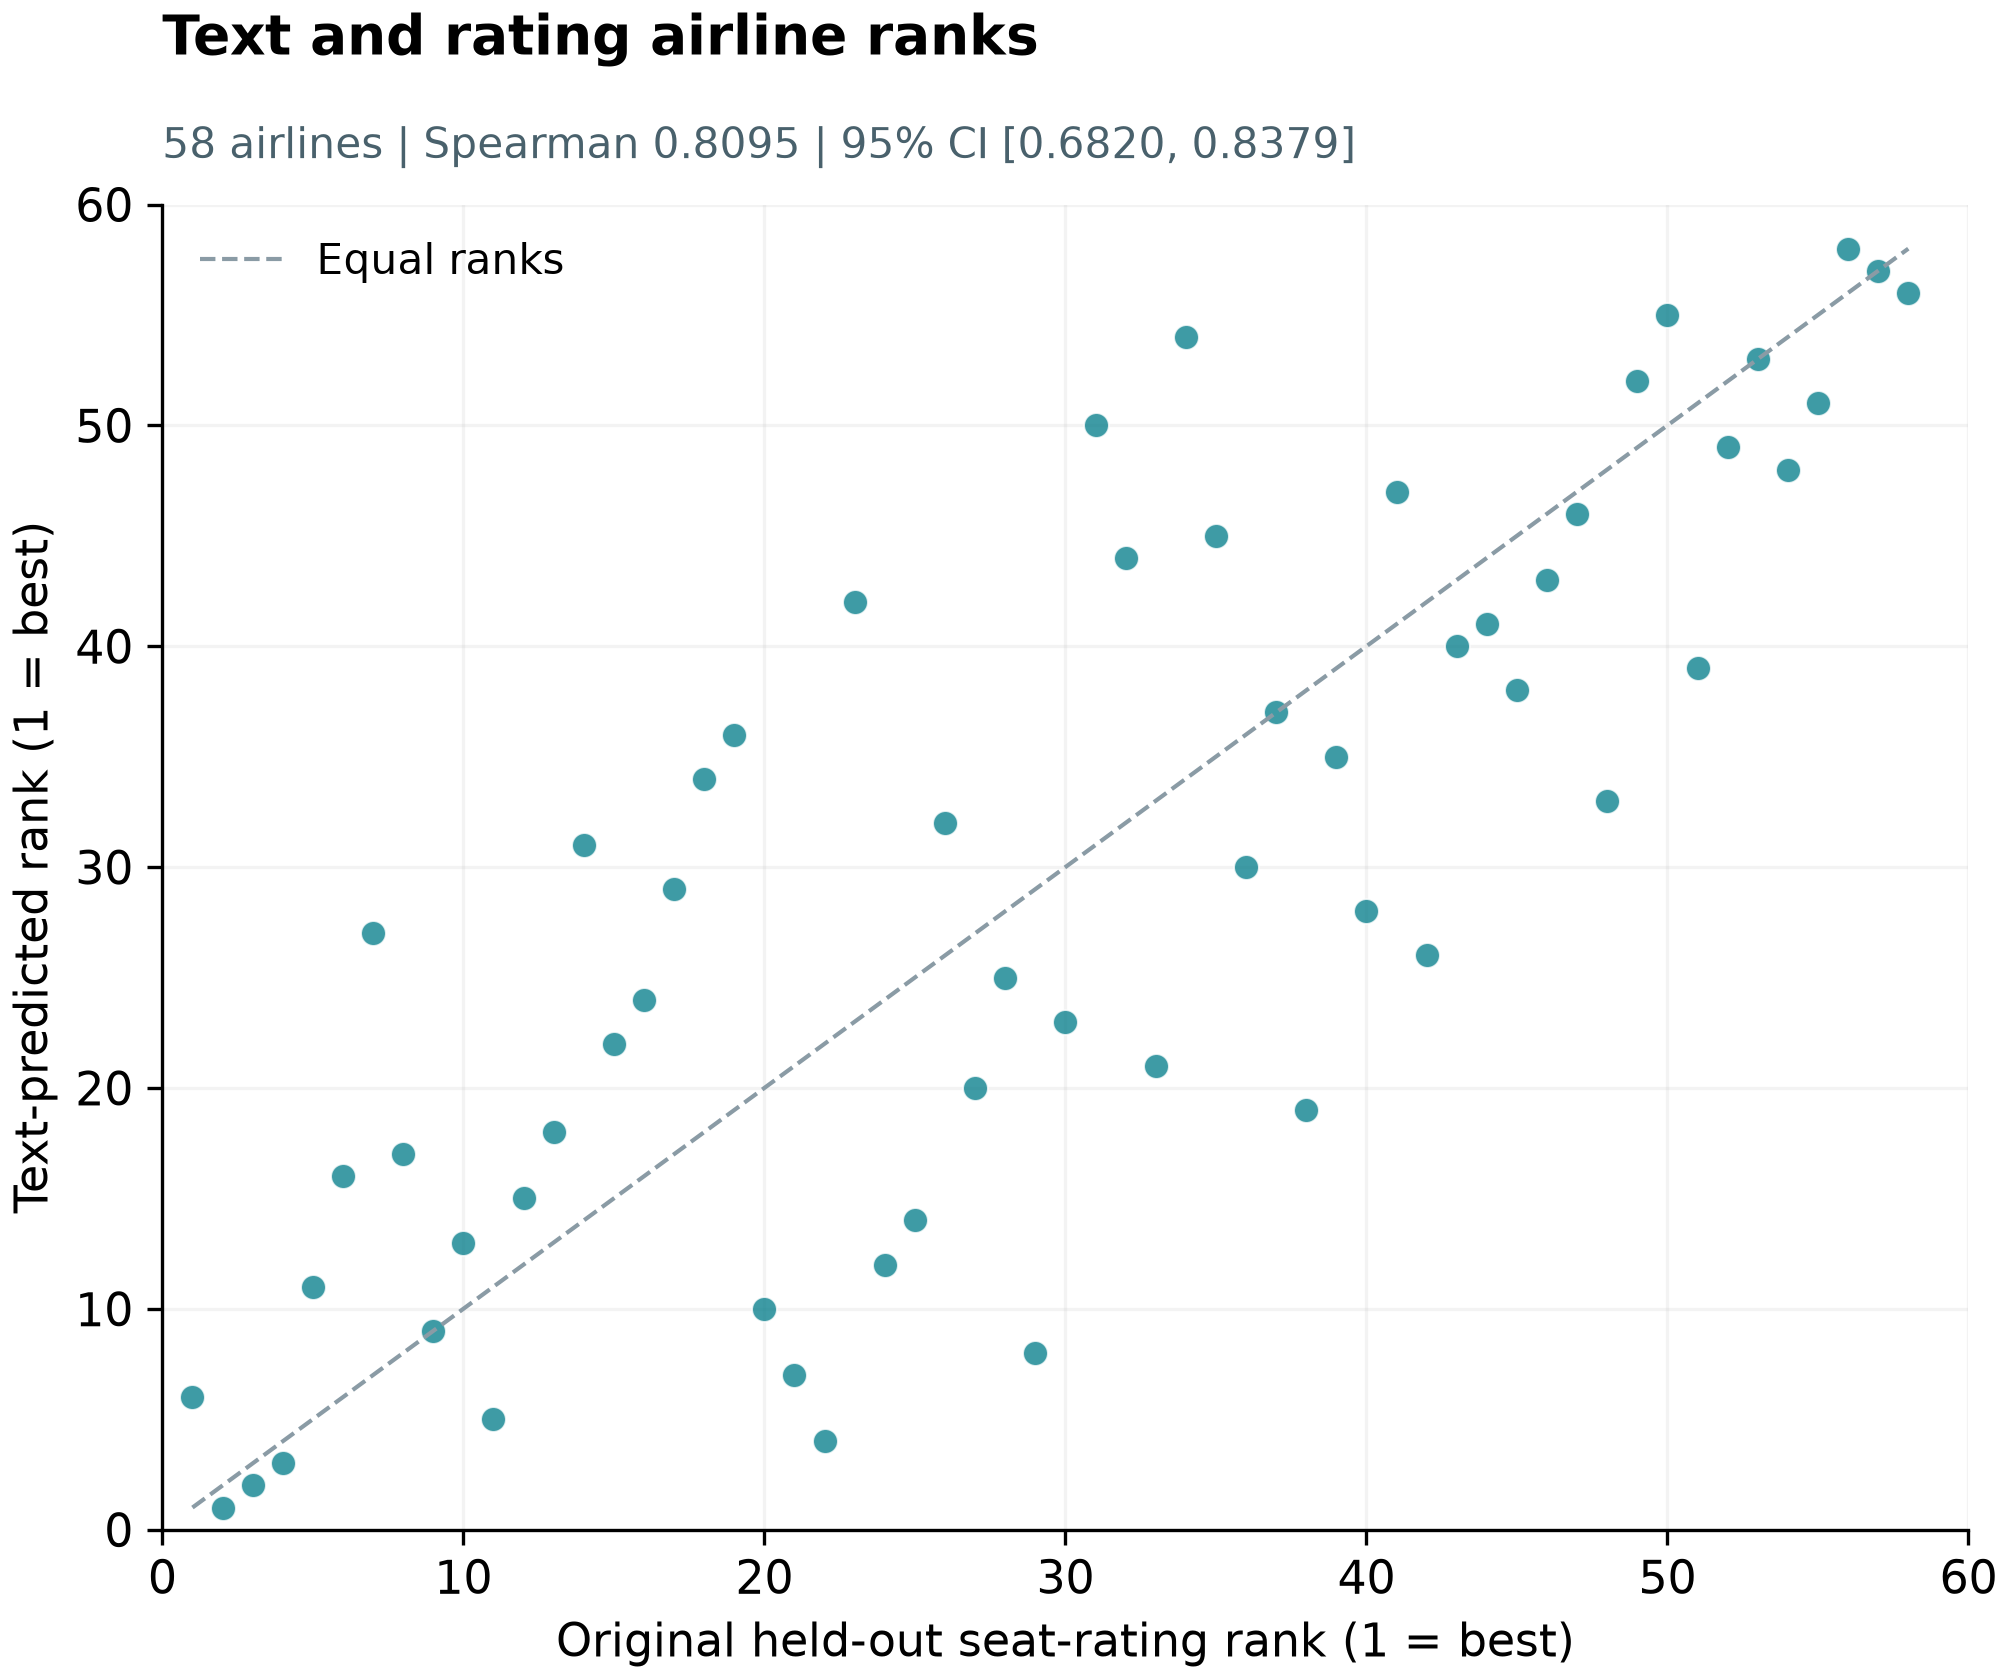
\includegraphics[width=\columnwidth, trim=0 0 0 46, clip]{figures/airline_rank_agreement.png}
\caption{E7: text-predicted vs.\ held-out rating rank for 58 airlines (1 = best); the dashed line marks equal ranks.
Spearman $\rho=0.810$, 95\% CI $[0.682, 0.838]$.}
\label{fig:rank}
\end{figure}

\paragraph{Results.} 58 airlines qualify. The held-out reference set holds \num{8365} reviews with a valid seat
rating, \num{3152} of them with a usable text prediction. The rankings agree closely: Spearman $\rho=0.810$, 95\% CI $[0.682,0.838]$, from 2,000
paired resamples of parent reviews over the fixed airline set (\cref{fig:rank}). Opinion mined from text and aggregated
per review therefore preserves clear differences between airlines, which supports using it for comparison questions.
The rating is a reference for overall seat comfort, not a gold standard for each sub-attribute, and the interval does
not include the uncertainty of retraining the classifier.

\subsection{E8: Performance and scalability (Q4)}
\label{sec:exp-perf}

\begin{table}[t]
\centering\small
\caption{E8: performance on an Apple M1 Pro (16\,GB). Query timings are medians (P95) over the 20 evaluation questions.}
\label{tab:perf}
\setlength{\tabcolsep}{3pt}
\begin{tabularx}{\columnwidth}{@{}Yr@{}}
\toprule
\textbf{Measure} & \textbf{Value} \\
\midrule
Retrieval and evidence selection & 2.9\,s (10.5\,s) \\
Submission to first streamed token & 24.3\,s (41.9\,s) \\
Submission to final checked answer & 40.8\,s (72.3\,s) \\
Program-only answer (LLM off) & 5.0\,s / query \\
Short LLM request (120 tokens), 1 or 2 at once & $\approx$1\,s each, serialised \\
\midrule
Student labelling of \num{529031} sentences & 18\,s \\
One-off MiniLM encoding of all sentences & 573\,s \\
LLM teacher labelling & $\approx$0.5\,s / sentence \\
KB rebuild / BM25 build / FAISS build & 14\,min / 6\,s / 4.6\,min \\
\midrule
Cost per query & \$0 (all local) \\
\bottomrule
\end{tabularx}
\end{table}

Retrieval and labelling scale well: indexes and labels are built offline, so query time depends on the filtered slice,
not on corpus size; the student labels $\approx$\num{30000} sentences per second (\cref{tab:perf}). Generation is the
bottleneck. Our single MLX server processes one request at a time, so two simultaneous users roughly double the wait;
serving more users needs several model workers or a GPU server with a batched engine such as vLLM. The 5\,s
program-only path is a usable fallback under load.

%--------------------------------------------------------------- Discussion
\section{Discussion and Limitations}
\label{sec:disc}

\paragraph{Automatic judges.} Retrieval relevance and RAG metrics are automatic, and the RAG judge is the generator
itself. An audit of the E6 judgements found 70 of 134 cached answer scorings listing more unsupported examples than the
number of unsupported claims they counted, and reordering the same passages changed context precision for one
question; bootstrap intervals do not capture such judge error. Human relevance judgements and blind human review of the
answers, ideally with an independent judge model, would strengthen E1, E5 and E6.

\paragraph{Small generator and strict checks.} 16 of 20 answers in E5 and 47 of 80 Z-on answers in E6 used the
program-written fallback; in Q01 of E6 a repair fixed a wrong number but changed the required wording of the statistics
sentence and was rejected. Separating semantic errors from format violations, and measuring the false-rejection rate,
is the next step; a larger local model or a short fine-tune on answers that passed the checks would also help.

\paragraph{Classifier below target.} Aspect F1 is 70.4 against a target of 85. Since teacher labels proved more valuable
per example than weak labels, the cheapest next steps are more teacher labels (30--50k sentences, a few GPU hours),
fine-tuning a small encoder on them, and a cascade that sends only low-confidence sentences to the LLM. Allowing more
than one aspect per sentence would also match the data better.

\paragraph{Airline names in English.} Late testing found ``\ldots Cathay Pacific or Singapore Airlines?'' parsed as a
single-airline question, because the corpus spells the name ``Cathay Pacific Airways''. A table of common English short
names now resolves this (it changes the parse of none of the evaluation questions); names outside the table still need
the corpus spelling, a Chinese name or the sidebar.

\paragraph{Data age.} Reviews end in mid-2019. The interface states this on every page; answers describe historical
experiences, not current service.

%--------------------------------------------------------------- Conclusion
\section{Conclusion}

We built a local RAG system for airline-service questions that keeps constraints, works at the level of fine-grained
attributes and gives verdicts a user can verify. Four lessons stand out. First, structured constraints and
attribute routing fixed the failing queries of \cref{tab:fixes}, which no change of ranking model addressed, and a
general-purpose cross-encoder even hurt. Second, distilling an LLM labeller into a linear classifier recovers most of its gain in objective detection and
about half of its gain in joint accuracy at a tiny fraction of its cost, provided selection is kept away from the test set. Third, balanced
evidence plus validation with a program-written fallback gives the most faithful final answers (Y + Z is the best of
eight configurations), but the gains are not additive: exact full-pool statistics fix the verdict while lowering judged
faithfulness. Finally, airline rankings mined from text agree with held-out passenger ratings ($\rho=0.81$), which
supports answering comparison questions from review text.

%--------------------------------------------------------------- Back matter
\section*{Data and Code Availability}
\addcontentsline{toc}{section}{Data and Code Availability}

\textbf{Release page:} \url{https://github.com/ntu-ai6127-g-13/ai6127-airline-rag/releases/tag/v1.0-submission}

\textbf{Data archive:} \url{https://github.com/ntu-ai6127-g-13/ai6127-airline-rag/releases/download/v1.0-submission/ai6127-g13-data.zip}\\
\nolinkurl{chunks.parquet} (knowledge base), \texttt{eval.xls} and the frozen gold CSV, the 20 evaluation questions with
retrieved evidence and generated answers, the 30-query retrieval benchmark with per-query results, label indexes
(v4.1 and distilled), classifier predictions on gold, teacher labels, the ablation case files, the factorial-ablation run (protocol, prompts, 160 answers, judge scores) and the
airline-ranking predictions.

\textbf{Code archive:} \url{https://github.com/ntu-ai6127-g-13/ai6127-airline-rag/archive/refs/tags/v1.0-submission.zip}\\
\nolinkurl{src/}, \nolinkurl{app/}, \nolinkurl{scripts/}, \nolinkurl{experiments/}, \nolinkurl{tests/},
\nolinkurl{requirements.txt} and a README with build and run instructions.

\section*{Contribution Statement}
All members contributed to the project. As recommended in the brief, we request a single grade shared by the whole
group.

\printbibliography

%--------------------------------------------------------------- Appendix
\appendix
\onecolumn
\section{Reproducing the Results}
\label{app:repro}

All commands run from the repository root with Python 3.11. Experiment scripts never overwrite earlier results: most
refuse an existing output directory, and the long-running ones resume from their checkpoints; the distillation scripts
also record SHA-256 hashes of their inputs.

\begin{Verbatim}[fontsize=\footnotesize, frame=single, framesep=3mm, rulecolor=\color{black!25}]
# environment and data (Q1)
python3.11 -m venv .venv && .venv/bin/pip install -r requirements.txt
.venv/bin/python -m spacy download en_core_web_sm
.venv/bin/python scripts/download_data.py
.venv/bin/python -m src.build_kb                       # about 14 min

# indexes
.venv/bin/python -m src.retriever build-bm25
.venv/bin/python -m src.retriever build-dense --batch-size 64
.venv/bin/python -m src.label_index --model outputs/weak_rebuild_20261019/model.joblib \
    --output-dir outputs/label_index_replay     # the archive already has label_index_20261019

# interface (Q2): local model server, then the app
.venv/bin/python scripts/setup_query_model.py           # once: pinned Qwen3-4B weights
outputs/query_quality_runtime/venv311/bin/python scripts/local_qa_server.py
.venv/bin/python scripts/run_query_app.py --port 8517

# retrieval benchmark and targeted checks (E1, E6); RAG metrics and latency (E2, E5)
.venv/bin/python -u experiments/final_auto_eval/run.py --output-dir outputs/final_auto_eval_replay
.venv/bin/python -u experiments/final_rag_eval/run.py --output-dir outputs/final_rag_eval_replay

# factorial ablation (E6) and airline ranking (E7): Linux GPU, Transformers backend;
# full commands in experiments/downstream_evaluation/README.md and FACTORIAL.md
.venv/bin/python scripts/local_qa_server.py --backend transformers --device cuda
P=outputs/downstream_protocol_replay
.venv/bin/python -m experiments.downstream_evaluation.freeze --output-dir $P
.venv/bin/python -m experiments.downstream_evaluation.ranking \
    --protocol $P/protocol.json --output-dir outputs/downstream_ranking_replay

# distillation (E3, E4); encode.py and evaluate_gold.py default to --device mps (use cpu/cuda
# elsewhere). The teacher step needs the MLX runtime and earlier r36 outputs, so the sample and
# its teacher labels ship in the data archive ($S); sample.py and label_teacher.py remake them.
D=experiments/distilled_label_index; O=outputs
S=$O/distill_sample_20261029; E=$O/distill_embeddings_20261029; R=$O/distill_students_replay
.venv/bin/python $D/encode.py --output-dir $E                                   # 5-10 min
.venv/bin/python $D/train_students.py --sample-dir $S --embeddings $E --output-dir $R
.venv/bin/python $D/evaluate_gold.py --selection $R/selection.json --output-dir $R/gold
.venv/bin/python $D/build_index.py --audit $R/gold/gold_audit.json \
    --selection $R/selection.json --embeddings $E --output-dir $O/label_index_distilled_replay
\end{Verbatim}

\section{Evaluation File Format}
\label{app:eval}

\texttt{eval.xls} (SHA-256 \texttt{fe0bcf0c…a477045}) is an Excel 97--2003 workbook written with \texttt{xlwt} from the
frozen gold CSV: one sheet, \num{1000} rows, no duplicate texts, and exactly the two benchmark columns \texttt{text} and
\texttt{label}. The gold CSV (\nolinkurl{data/eval/gold_human_frozen_1000_20261019_v1.csv}) has the same rows in the same
order and adds the step-wise labels and provenance:

\begin{center}\small
\begin{tabularx}{\textwidth}{@{}P{34mm}P{52mm}Y@{}}
\toprule
\textbf{Column} & \textbf{Values} & \textbf{Meaning} \\
\midrule
\texttt{text} & string & The sentence, exactly as shown to annotators. \\
\texttt{label} & objective / positive / negative & Three-class sentiment label (benchmark format). \\
\texttt{subjectivity} & objective / subjective & Step 1 of the task. \\
\texttt{polarity} & positive / negative / NA & Step 2; \texttt{NA} for objective sentences (read with \nolinkurl{keep_default_na=False}). \\
\texttt{aspect} & seat, staff, food, entertainment, ground, value, overall, other & Aspect the sentence is about. \\
IDs and provenance & sentence, review and chunk IDs; review status & Joins back to the knowledge base; audit trail of the human review. \\
\bottomrule
\end{tabularx}
\end{center}

\paragraph{Question sets.} \nolinkurl{data/eval/query_smoke_40_20261019.json} is a JSON array of 40 questions, each
with \texttt{id}, \texttt{language}, \texttt{question}, the expected \texttt{aspect}/\texttt{aspects}, the expected
\texttt{subtopics} (sub-attributes) and a \texttt{comparison} flag. E1 parses Q01--Q25 into the 30 airline $\times$
sub-attribute units; E2 and E5 use Q01--Q12, Q21--Q25 and Q28--Q30. Results are JSONL with one record per question
(\texttt{case}, \texttt{parsed}, \texttt{result} with the retrieved evidence and timings, \texttt{answer} with text,
mode and citations, and \texttt{judge}), or CSV with one row per query and method.

\section{The Queries of Table~\ref{tab:five}: Wording and Results}
\label{app:queries}

Counts are reviews that directly match the attribute; percentages are over those with a clear direction. Full answers,
with citations and evidence, are in \nolinkurl{outputs/final_rag_eval_20261019/answers.jsonl}.

\begin{center}\small
\begin{tabularx}{\textwidth}{@{}lP{62mm}Y@{}}
\toprule
\textbf{ID} & \textbf{Question as asked} & \textbf{Result} \\
\midrule
Q05 & 阿联酋航空经济舱的退款和改签处理怎么样？ & Negative: 19 of 19 directional reviews (24 matches) negative; cites unpaid refunds after repeated contact and cancellation and seat fees. \\
Q10 & 卡塔尔航空商务舱的电影选择和娱乐内容怎么样？ & Mixed: 15 positive, 15 negative (86 matches); a wide film selection versus dated content and poor TV choice. \\
Q24 & 国泰航空和新加坡航空经济舱腿部空间哪家评价更好？ & No clear winner on legroom: Cathay Pacific 72.5\% positive (50/69), Singapore Airlines 79.6\% (78/98); Singapore's seat rating is higher (3.83 vs.\ 3.46 of 5). \\
Q28 & 新加坡航空经济舱的腿部空间、靠背调节、座椅舒适度和座椅清洁度分别怎么样？ & Legroom positive (78/98, 79.6\%); recline mixed (14/26); seat comfort positive (97/123, 78.9\%); cleanliness too few to decide (7/10). \\
Q30 & 新加坡航空经济舱的餐食、性价比和地面服务分别怎么样？ & Food 65.5\% positive (289/441, rating 3.88); value 34.6\% positive (75/217, rating 3.88); ground service 43.6\% positive (163/374, rating 3.99). \\
\bottomrule
\end{tabularx}
\end{center}

\section{Questions of the Factorial Ablation}
\label{app:factorial}

Each question reads ``What do historical reviews say about [attribute] on [airline] in [cabin]?''. These IDs are
local to E6 and unrelated to the IDs of \cref{tab:five}.

\begin{center}\small
\begin{tabular}{@{}llll@{\hspace{10mm}}llll@{}}
\toprule
\textbf{ID} & \textbf{Airline} & \textbf{Cabin} & \textbf{Attribute} & \textbf{ID} & \textbf{Airline} & \textbf{Cabin} & \textbf{Attribute} \\
\midrule
Q01 & Singapore Airlines & Economy & legroom & Q11 & British Airways & Prem.\ Econ. & recline / lie-flat \\
Q02 & Air Canada rouge & Economy & legroom & Q12 & Cathay Pacific & Business & staff attitude \\
Q03 & Spirit Airlines & Economy & baggage & Q13 & United Airlines & Economy & seat width \\
Q04 & Alaska Airlines & Economy & delay handling & Q14 & Turkish Airlines & Economy & food quality \\
Q05 & Emirates & Economy & refunds / changes & Q15 & AirAsia & Economy & customer support \\
Q06 & Singapore Airlines & Economy & meal variety & Q16 & Etihad Airways & Business & recline / lie-flat \\
Q07 & Singapore Airlines & Economy & portion size & Q17 & Frontier Airlines & Economy & baggage \\
Q08 & Singapore Airlines & Economy & seat cleanliness & Q18 & American Airlines & Economy & check-in \\
Q09 & Emirates & Economy & Wi-Fi & Q19 & Lufthansa & Economy & punctuality \\
Q10 & Qatar Airways & Business & entertainment & Q20 & Qantas Airways & Economy & drinks \\
\bottomrule
\end{tabular}
\end{center}

\section{Aspect and Sub-attribute Taxonomy}
\label{app:taxonomy}

\begin{center}\small
\begin{tabularx}{\textwidth}{@{}P{30mm}Y@{}}
\toprule
\textbf{Aspect} & \textbf{Sub-attributes (46 in total)} \\
\midrule
Seat & legroom, width, recline and lie-flat, comfort, condition, seat cleanliness, power, privacy, storage \\
Food & specific dishes, quality and taste, portion size, variety, drinks, special meals, temperature, meal-service process \\
Entertainment & content, screen, Wi-Fi, headphones and audio, system usability \\
Staff & attitude, efficiency, professionalism, availability, communication and language \\
Ground & punctuality, delay and cancellation handling, baggage, check-in, gate and boarding, lounge, connections, special assistance \\
Value & ticket price, refunds and changes, customer support, booking system, additional fees \\
Other & cabin cleanliness, lavatory, cabin temperature, amenities, cabin noise, aircraft and cabin condition \\
Overall & whole-trip judgements; no sub-attributes \\
\bottomrule
\end{tabularx}
\end{center}

\end{document}
